% 理论章节以任务后果统一B/C/D；当前方法仍为动作与几何监督，不含任务价值学习。
\documentclass[journal,10pt]{IEEEtran}
\usepackage{amsmath,amssymb,bm,mathtools,booktabs,array}
\usepackage{graphicx}
\usepackage{xeCJK}
\setmainfont{NimbusRoman}[
 Path=/usr/share/fonts/opentype/urw-base35/,
 Extension=.otf,UprightFont=*-Regular,BoldFont=*-Bold,
 ItalicFont=*-Italic,BoldItalicFont=*-BoldItalic,SmallCapsFont=*-Regular]
\setCJKmainfont[AutoFakeBold=true,AutoFakeSlant=true,SmallCapsFont={Droid Sans Fallback}]{Droid Sans Fallback}
\setCJKsansfont{Droid Sans Fallback}
\setCJKmonofont{Droid Sans Fallback}
\usepackage{xeCJKfntef}
\usepackage{algorithmic}
\usepackage{tikz}
\usepackage{placeins}
\usetikzlibrary{arrows.meta}
\usepackage{cite}
\usepackage{comment}
\usepackage[hidelinks]{hyperref}
\newcommand{\draftnote}[1]{\par\smallskip{\small（\CJKunderline{#1}）}\par\smallskip}
\newcommand{\E}{\mathbb E}
\newcommand{\Prob}{\mathbb P}
\newcommand{\R}{\mathbb R}
\newcommand{\norm}[1]{\lVert#1\rVert}
\newcommand{\inner}[2]{\langle#1,#2\rangle}
\newcommand{\ind}{\mathbf 1}
\DeclareMathOperator{\clip}{clip}
% \newtheorem{proposition}{命题}
\newtheorem{proposition}{Proposition}
% \newtheorem{assumption}{假设}
\newtheorem{assumption}{Assumption}
\renewcommand{\IEEEproofname}{证明}
\renewcommand{\refname}{参考文献}
\title{Bimanual Exposure and Execution via Task-Aware Imitation Learning}
\author{}
\makeatletter
\let\tableinput\@@input
\makeatother
\begin{document}
\maketitle
\begin{abstract}
Bimanual exposure and execution under deformable occlusion require a robot to reveal an initially hidden target, manipulate it into a designated region, and restore the covering while adapting later actions to the outcomes of earlier interactions. Conventional visuomotor imitation learning primarily supervises action prediction and may therefore fail to preserve the task information needed to determine whether exposure is sufficient and how execution should proceed. We present a task-aware imitation learning framework that explicitly encourages the policy representation to retain target visibility and interaction geometry. A quality-aware iterative annotation procedure expands semantic supervision from a small set of reviewed videos. The resulting semantic maps provide object-level visual structure, while supervised query tokens encode task descriptors, including target visibility, tool--target displacement, and target--goal distance, jointly with action-chunk prediction. We further derive conditions linking imitation error and representation quality to complete-task failure. Our real-robot evaluation comprises 480 trials across five policies, four object types, and 12 initial positions using the same fixed demonstration set. The proposed method succeeds in 92 of 96 trials (95.8\%), compared with 54 of 96 (56.2\%) for ACT and 50 of 96 (52.1\%) for Diffusion Policy. Factorial ablations achieve 60 of 96 trials with semantic inputs alone and 72 of 96 with supervised queries alone, while their combination performs best. These results show that explicitly preserving task-relevant information can substantially improve complete-task execution from limited demonstrations.
\end{abstract}
\begin{IEEEkeywords}
Imitation learning, semantic representations, visuomotor control.
\end{IEEEkeywords}
\section{Introduction}
\label{sec:intro}

Robots frequently need to change a scene before the intended operation becomes feasible. We study a class of \emph{bimanual exposure-and-execution} tasks in which one or both arms first manipulate a deformable occluder to reveal a target, subsequently operate on the target, and finally restore the surrounding scene. This structure appears in everyday activities, such as lifting a cloth to remove an object underneath and replacing the cloth, and in surgery, where tissue retraction establishes visibility and access for a subsequent intervention~\cite{attanasio2020retraction,pore2021retraction}. These tasks are sequential, but their difficulty is not merely the length of the action sequence: the outcome of each operation establishes, or destroys, the physical and perceptual conditions required by the next. Related dependencies arise in manipulation-based object search~\cite{dogar2014search,danielczuk2019mechanical} and preparatory manipulation~\cite{wan2020preparatory,shen2026bipremanip}. Figure~\ref{fig:taskoverview} shows the complete task considered here, from exposure through target manipulation to restoration.

\begin{figure}[t]
\centering
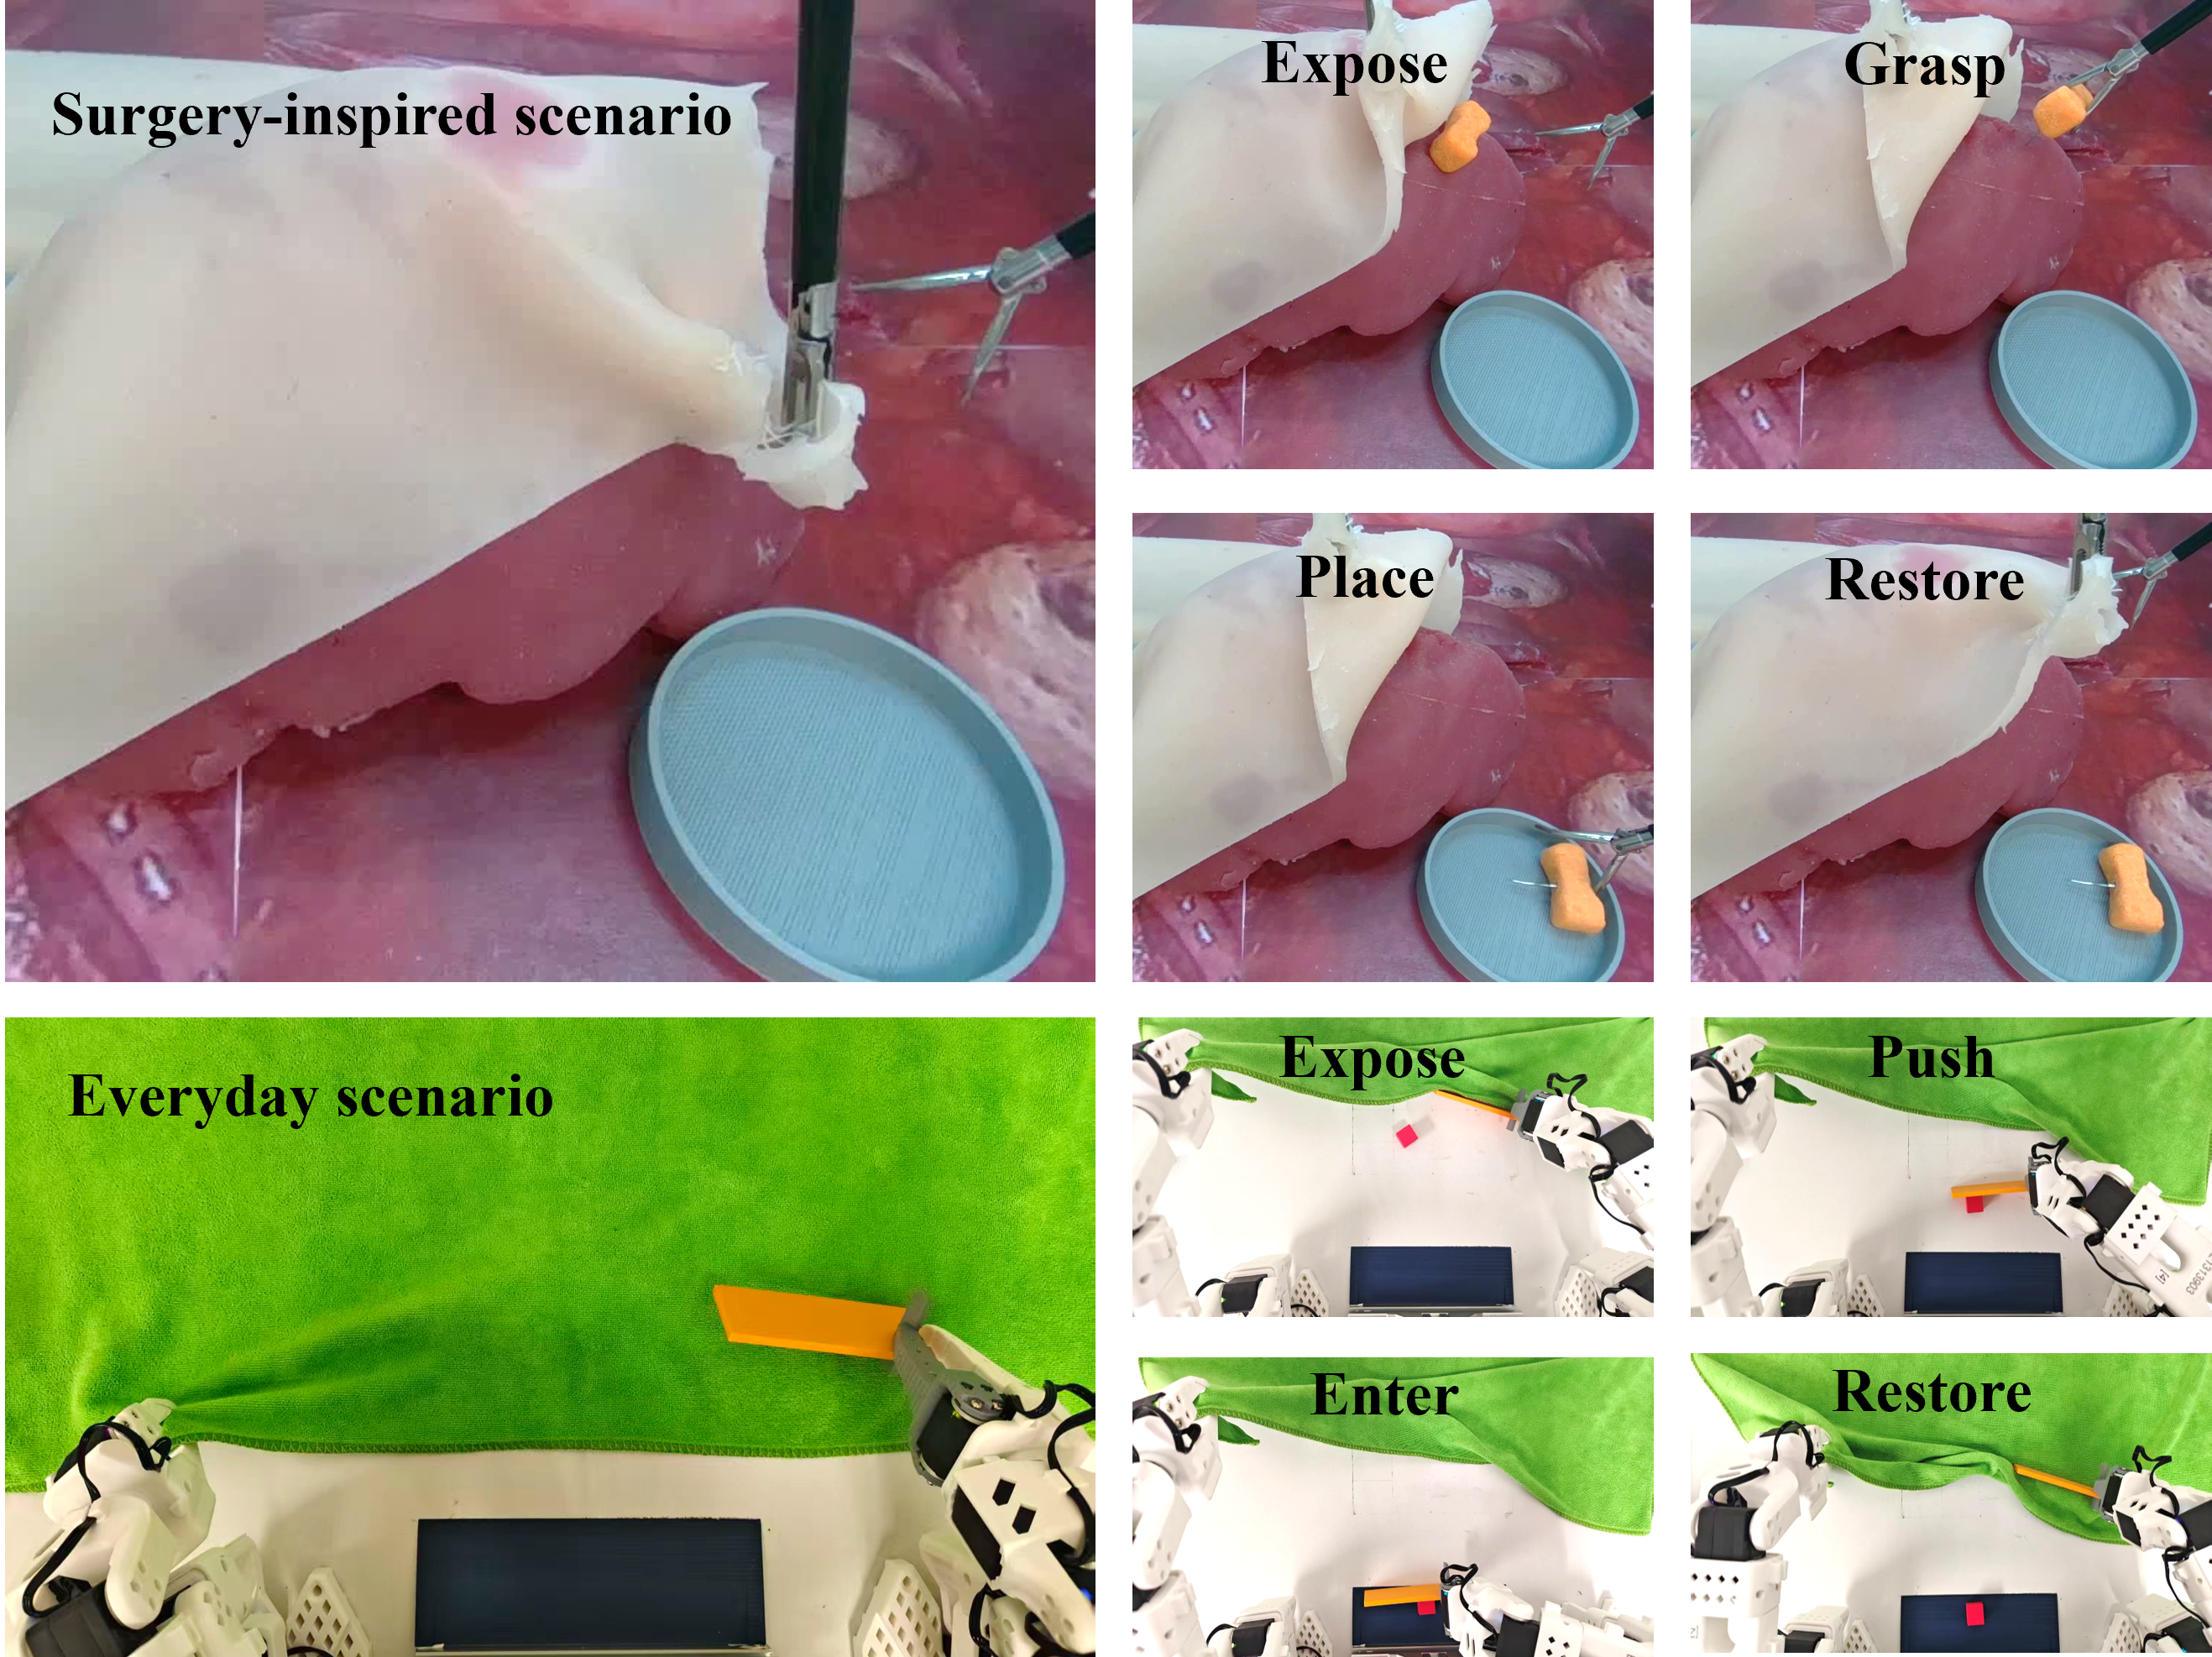
\includegraphics[width=\columnwidth]{myfigure/taskoverview1.png}
\caption{Overview of our bimanual exposure-and-execution tasks. The robot needs to expose an occluded target, manipulate it into a designated region, and restore the deformable covering by executing the sequences of operations displayed on the right.}
\label{fig:taskoverview}
\end{figure}

Exposure and execution couple perception, contact, and coordination in ways that make complete-task success substantially harder than performing the visible terminal operation alone. A deformable covering has a high-dimensional configuration and can fold, slip, or re-occlude the target after contact. The two arms take changing and often asymmetric roles: one arm may maintain or enlarge the exposed region while the other approaches the target, after which both must coordinate target transfer and restoration. Moreover, exposure is not a binary, isolated subgoal. An action can reveal part of the target yet leave insufficient tool clearance, displace the target, or place the occluder where it obstructs a later motion. The policy must therefore use visual feedback to track task conditions---including target visibility and the spatial relationships among the occluder, tools, target, and goal---and adapt later actions to the actual outcome of earlier interactions. Because complete success requires all of these conditions to remain compatible, a locally plausible action can still cause failure several operations later.

Visuomotor imitation learning is attractive for such contact-rich tasks because it can learn perception and control directly from demonstrations without an explicit model of deformable-object dynamics. Action Chunking with Transformers (ACT) learns temporally coherent bimanual commands~\cite{zhao2023act}, while Diffusion Policy represents multimodal action sequences through conditional denoising~\cite{chi2023diffusion}. These policy classes have enabled coordinated and multistage behaviors in systems such as Mobile ALOHA and UMI~\cite{fu2024mobilealoha,chi2024umi}. Explicit temporal abstractions provide another route: sequential manipulation can be represented with learned primitives or geometric constraints~\cite{liang2022sensorimotor,perez2017clearn}, and hierarchical policies can select, retry, and compose skills over long horizons~\cite{gupta2020relay,luo2024cable}. In this work, we ask a complementary question: when learning a single closed-loop action-chunk policy from a fixed and limited demonstration set, what information should its representation preserve so that subsequent actions remain compatible with the evolving task state?

Standard behavior cloning answers this question only indirectly through action-prediction loss. This is problematic for two related reasons. First, small errors can move the robot to histories that are weakly represented in the demonstrations, after which error compounds over the remaining horizon~\cite{ross2011,laskey2017dart}. Second, low demonstration loss does not by itself identify why the expert selected an action. A high-capacity policy may exploit visual or temporal correlations that predict demonstrated commands while omitting the physical relations that determine whether those commands remain appropriate; this issue is closely related to causal confusion and copycat behavior in imitation learning~\cite{dehaan2019,wen2020copycat}. Supplying object-centric features or semantic channels can reduce visual complexity, but their presence at the input does not guarantee that the internal representation used for action generation retains the particular visibility and geometric relations needed by the task. This distinction is especially consequential in exposure-and-execution tasks, where similar arm configurations can require different continuations depending on what the preceding interaction actually exposed or displaced.

We therefore use \emph{task-aware imitation learning} in a specific, operational sense: in addition to matching expert actions, the policy is trained so that selected task conditions remain recoverable from the representation that generates those actions. Our framework derives semantic masks for task entities and converts them into descriptors of target exposure and interaction geometry, including visible area, tool--target displacement, and target--goal distance. Learnable task queries integrate visual and proprioceptive observations; descriptor heads supervise the encoded query tokens, which are also available to the action decoder. This design differs from merely appending a segmentation image: semantic inputs provide object-level structure, whereas query supervision explicitly encourages the action-generating representation to preserve chosen task information. Because dense labels are costly, a quality-aware iterative annotation procedure expands three manually reviewed seed trajectories into semantic supervision over 102 additional trajectories, retains three disjoint trajectories for diagnostic monitoring, and uses temporal and structural tests to screen unreliable pseudo-labels.

The representation design is motivated by a task-level analysis rather than by the assumption that semantics automatically improve control. We first relate coordinated action error over the interaction horizon to complete exposure-and-execution failure. We then separate two requirements for transferring performance from demonstrations to deployment: coverage of deployment histories in the learned representation and preservation of information from which expert bimanual commands can be reconstructed. The resulting conditional bounds clarify both the intended benefit and the limitation of descriptor supervision: it targets a measurable representation error term, but successful execution still depends on coverage, action sensitivity, and whether the selected descriptors adequately explain expert choices.

We evaluate all policies using the same fixed set of 108 real-robot demonstrations. The test comprises 480 trials across five policies, four object types, and 12 initial positions. Our full method succeeds in 92 of 96 trials (95.8\%), compared with 54 of 96 (56.2\%) for ACT and 50 of 96 (52.1\%) for Diffusion Policy. In a $2\times2$ factorial ablation, semantic inputs alone reach 60 of 96 successes and supervised task queries alone reach 72 of 96; combining them yields the strongest complete-task performance. The improvement is achieved without additional policy interaction data and without introducing an explicit phase label or hierarchical skill selector.

The main contributions of this work are:
\begin{itemize}
    \item a formulation of bimanual exposure and execution that makes the dependence of later operations on achieved visibility and interaction geometry explicit, together with an analysis connecting action error and representation quality to complete-task failure;
    \item a task-aware visuomotor imitation framework that combines semantic observations with descriptor-supervised query tokens, directly encouraging task information to remain recoverable from the action-generating representation;
    \item a quality-aware iterative annotation procedure that expands sparse reviewed video masks into descriptor supervision while screening temporal and structural anomalies; and
    \item a controlled real-robot evaluation with 480 trials, including policy comparisons, factorial ablations, stage-wise outcomes, and a held-out object category, showing that semantic inputs and task-query supervision are complementary.
\end{itemize}

\section{Related Work}
\label{sec:relatedwork}

\subsection{Exposure, Preparatory, and Deformable-Object Manipulation}

Robotic manipulation often includes actions whose purpose is to establish conditions for a later operation. Manipulation-based object search reasons about visibility and reachability while moving occluding objects~\cite{dogar2014search}; mechanical search combines repeated perception and pushing, suction, or grasping to retrieve a target hidden in clutter~\cite{danielczuk2019mechanical}. Preparatory-manipulation planners instead regrasp, place, or hand over an object to reach a configuration suitable for later use~\cite{wan2020preparatory}. Recent BiPreManip learns anticipatory affordances for asymmetric bimanual tasks in which one arm reconfigures an object for the other arm's goal-directed operation~\cite{shen2026bipremanip}. These works establish the importance of actions that make later manipulation feasible. Mechanical search primarily removes rigid clutter to find or retrieve a target, while preparatory manipulation primarily changes the configuration of the manipulated object. Our setting combines physical exposure, target execution, and restoration under a deformable occluder, and evaluates whether a continuous visuomotor policy preserves the changing conditions connecting these operations.

Occlusion can also be addressed by changing sensing rather than changing the scene. Active-vision systems move a camera to improve task-specific viewpoints for bimanual imitation learning~\cite{chuang2025activevision}. In contrast, exposure in our tasks is itself a contact-rich manipulation objective: moving the occluder changes both what can be observed and what motions are physically feasible. Surgical tissue retraction provides a particularly relevant example. Prior systems study autonomous retraction with engineered perception and control~\cite{attanasio2020retraction}, learning from demonstrations~\cite{pore2021retraction}, or adaptive visual control for exposing a region of interest~\cite{liu2026exposure}. These approaches focus on attaining and maintaining exposure. We study the broader dependency between exposure and the subsequent target operation, including restoration as part of the complete-task criterion.

Deformable-object manipulation is challenging because cloth, rope, tissue, and bags have high-dimensional configurations, complex contact dynamics, and perceptual ambiguity~\cite{jimenez2012deformable,sanchez2018deformable}. Model-based methods encode object geometry and mechanics, whereas data-driven methods learn state estimates, dynamics, or policies from interaction data. Representative learning-based systems acquire visual policies for cloth and rope manipulation without demonstrations~\cite{wu2020deformable}, combine goal-conditioned local and global actions for deformable objects~\cite{kim2024dualaction}, or learn structure-of-interest dynamics for bimanual bag manipulation~\cite{zhou2025bag}. Rather than reconstructing or predicting the complete deformable state, our method selects task descriptors that summarize visibility and spatial relationships needed for action selection. This is a deliberate abstraction: RGB and proprioception remain available for contact and deformation cues not represented by those descriptors.

\subsection{Visuomotor Imitation for Sequential and Bimanual Manipulation}

Visuomotor imitation learning maps sensory observations and robot state to actions without requiring an explicit contact model. Modern policies often predict temporally extended commands. ACT uses a transformer to generate action chunks for fine-grained bimanual manipulation~\cite{zhao2023act}, whereas Diffusion Policy models multimodal action sequences through conditional denoising~\cite{chi2023diffusion}. These policy families support coordinated and multistage behaviors in Mobile ALOHA and UMI~\cite{fu2024mobilealoha,chi2024umi}. Recent work also improves bimanual data efficiency by extracting reusable motion patterns from human videos and learning a bimanual diffusion policy~\cite{zhou2025yoto}. Such methods provide strong action-generation backbones, but action prediction alone does not specify which consequences of earlier interactions should remain explicit in the policy representation.

Long-horizon manipulation can instead be organized with explicit task structure. Neural task programs and learned sensorimotor primitives decompose demonstrations and select skills using visual state, object relations, or action history~\cite{xu2018ntp,liang2022sensorimotor}. C-LEARN represents multistep demonstrations as ordered keyframes with geometric constraints~\cite{perez2017clearn}, while Relay Policy Learning uses goal-conditioned hierarchical policies initialized from unstructured demonstrations and refined with reinforcement learning~\cite{gupta2020relay}. For physical multistage tasks, hierarchical imitation has been used to select and retry primitives for cable routing~\cite{luo2024cable}, and dual-action imitation combines reactive local commands with generated global trajectories for deformable-object manipulation~\cite{kim2024dualaction}. These approaches address temporal abstraction, skill sequencing, constraint satisfaction, or trajectory generation. Our work keeps a single action-chunk policy and fixed offline demonstrations, and instead studies whether the representation used by that policy retains achieved exposure and interaction geometry. It consequently requires neither primitive annotations nor an explicit phase, subgoal, or high-level skill selector.

\subsection{Task-Relevant Representations for Imitation Learning}

Behavior cloning can fit demonstrated actions using correlations that are predictive in the dataset but unreliable during closed-loop execution. Causal-confusion analyses show that an imitation learner can select the wrong causal explanation for expert behavior~\cite{dehaan2019}. With observation histories, policies can similarly copy preceding actions rather than use environmental evidence; adversarial history dropout and residual-action prediction were developed to counter this shortcut~\cite{wen2020copycat,chuang2022rap}. These studies concern temporal or causal shortcuts rather than exposure geometry specifically, but they motivate our central distinction: small action-prediction error does not guarantee that the learned representation preserves the physical information on which an appropriate action depends.

Structured visual representations reduce the burden of extracting such information from pixels. Transporter Networks encode pick-and-place geometry through feature transport~\cite{zeng2021transporter}; VIOLA uses object proposals and attention to emphasize regions useful for action generation~\cite{zhu2023viola}; and GROOT learns object-centric 3-D representations for generalization across scenes and instances~\cite{zhu2023groot}. SAM-E adapts a visual foundation model to extract task-relevant features for sequence imitation~\cite{zhang2024same}. More recently, task-aware semantic--geometric observation interfaces use open-vocabulary segmentation and depth to canonicalize policy inputs under appearance shifts~\cite{ding2026choose}. These methods demonstrate the value of spatial and object-centric priors. Our method further constrains internal action-generating queries so that selected task descriptors are recoverable; the ablations therefore separate the effect of supplying semantic observations from the effect of supervising what the joint policy representation retains.

Task awareness has also been introduced through learning objectives and additional teaching signals. Belief-module imitation learning jointly trains a history representation and an adversarial policy with a task-aware imitation loss~\cite{gangwani2020belief}. TRAIL restricts an adversarial-imitation discriminator to avoid spurious task-irrelevant visual features~\cite{zolna2021trail}, while information-bottleneck behavior cloning suppresses latent redundancy while preserving features useful for manipulation~\cite{bai2025ibbc}. CIVIL asks demonstrators to identify decision-relevant objects and positions through language and physical markers, then learns a compact causal visual representation with the policy~\cite{dai2026civil}. TARAD uses language-model planning and visual affordances to generate demonstrations for a multitask diffusion policy~\cite{hu2025tarad}. Thus, \emph{task-aware imitation learning} is not introduced here as a new general term. In our setting it has a narrower operational definition: mask-derived descriptors of target visibility, tool--target displacement, and target--goal distance are supervised directly from policy query tokens and trained jointly with action prediction. They are neither task identifiers nor reward or discriminator features; they state what physical information should remain readable from the representation producing coordinated bimanual commands.

Our descriptor targets depend on scalable semantic supervision. Promptable video segmentation models such as SAM2 propagate sparse prompts through video~\cite{ravi2024sam2}, and semi-supervised segmentation methods expand sparse labels using consistency-based pseudo-labeling~\cite{yang2023unimatch}. Because persistent segmentation errors can yield plausible yet incorrect geometric descriptors, our workflow combines reviewed bidirectional masks with video-level temporal and structural screening before cumulative self-training. This annotation procedure supplies supervision to the policy; it is not itself assumed to improve control, and its effect is evaluated through the downstream factorial ablation.

\subsection{Distribution Shift and Task-Level Analysis}

Behavior cloning can accumulate errors when a learned policy visits states that are poorly represented in demonstrations. DAgger addresses this distribution shift by querying the expert on learner-visited states~\cite{ross2011}, whereas DART perturbs demonstrations to collect behavior around likely execution errors~\cite{laskey2017dart}. These approaches improve deployment coverage but require additional expert interaction or a modified collection process. Our method retains a fixed demonstration set and examines how task-directed representation supervision changes the policy learned from it; it does not claim to eliminate unsupported deployment histories.

Several analyses connect local imitation decisions to longer-term performance. AggreVaTe and value aggregation evaluate actions through downstream task cost~\cite{ross2014aggrevate,cheng2018value}, while stability-constrained imitation learning and TaSIL control error propagation under regularity assumptions on the system and expert~\cite{tu2022,pfrommer2022tasil}. Representation and domain-adaptation analyses further show that distribution alignment can discard information needed for prediction unless support and recoverability conditions are preserved~\cite{johansson2019support,zhao2019invariant}. Our analysis complements these results. Under explicit coverage and action-sensitivity conditions, it connects representation-level imitation error to failure of the complete exposure-and-execution task and gives expert-action reconstruction from task descriptors as a sufficient route for controlling the demonstration-to-deployment error discrepancy. These are conditional design guarantees, not an assertion that semantic supervision alone ensures task success.

\section{Problem Formulation and Theoretical Analysis}
\label{sec:analysis}
% 本章分析有限示范下双臂暴露与执行任务的改进条件。
This section studies conditions for improving bimanual exposure and execution from limited demonstrations.
% 暴露动作改变后续操作条件，因此以完整任务后果分析双臂动作偏差。
Because interactions with an occluder change the conditions for subsequent execution, we relate deviations in coordinated actions to failure of the complete task.
% 先由动作误差得到任务界，再说明表示覆盖本身不足以控制该界。
We first derive a task-failure bound under coverage and action-sensitivity conditions, then show why improved representation-level coverage alone is insufficient.
% 再分析可见性与空间关系何时保留专家选择依据，并通过动作重构约束误差迁移。
We next examine when visibility and spatial relationships preserve information needed for expert choices, linking their estimation accuracy to expert-action reconstruction and conditional error transfer.
\subsection{Bimanual Exposure and Execution}
\label{sec:task}

We study bimanual exposure and execution under deformable occlusion.
The arms first establish visibility and access to an occluded target, then complete a prescribed operation and any required restoration.
Because exposure can change both the occluder configuration and target state, subsequent actions must respond to the resulting interaction conditions.
We learn from a finite, fixed demonstration set and evaluate complete-task success within a finite horizon using visual history.

\subsubsection{System, Demonstrations, and Policy}

A single policy coordinates both arms, whose roles may change during execution.
The joint robot-environment state $s_t\in\mathcal S$ includes the arms, target, deformable occluder, and their interaction conditions.
The joint command $u_t\in\mathcal A\subseteq\R^{d_u}$ controls both arms and their end effectors.
The observation $o_t=(I_t^{1:V},\mathbf{x}_t^{\mathrm{prop}})$ contains images from $V\ge1$ cameras and the proprioceptive state $\mathbf{x}_t^{\mathrm{prop}}$.
Over $T$ control steps, the interaction follows
\begin{align}
 s_0&\sim p_0,\nonumber\\
 s_{t+1}&\sim P(\cdot\mid s_t,u_t),\quad 0\le t<T,\nonumber\\
 o_t&\sim O(\cdot\mid s_t),\quad 0\le t\le T.
 \label{eq:interactionmodel}
\end{align}
where $p_0$ is the initial-state distribution and $P$ and $O$ are the transition and observation kernels.
The transition kernel captures coupled arm motion, occluder deformation, and target interaction.

The fixed demonstration set $\mathcal D=\{\zeta_i\}_{i=1}^{N}$ records observations and expert commands for the same task objective:
\begin{equation}
 \zeta_i=(o_0^i,u_0^{\mathrm E,i},o_1^i,\ldots,
 u_{T_i-1}^{\mathrm E,i},o_{T_i}^i).
 \label{eq:demonstrations}
\end{equation}
Here, $T_i$ is the length of trajectory $i$ and the superscript $\mathrm E$ denotes expert commands.
For the analysis, the deployed policy is deterministic and selects $u_t=\pi(\mathcal H_t)$ from the available history $\mathcal H_t$, which contains observations $o_{0:t}$, past commands $u_{0:t-1}$, and any runtime context available before the current decision.

\subsubsection{Learning and Task Objectives}
Let $\pi_{\mathrm E}$ denote the expert policy and let $\nu$ be the population distribution of uniformly sampled demonstration control steps and their histories.
This uses the same control-step weighting as the deployment average introduced below.
The population imitation risk is
\begin{equation}
 R_\nu(\pi)
 :=\E_{(t,h)\sim\nu}\norm{\pi(h)-\pi_{\mathrm E}(h)}^2.
 \label{eq:populationimitationrisk}
\end{equation}
The empirical objective in Section~\ref{sec:method} uses a masked $L_1$ surrogate for this expert-action discrepancy.

The measurable completion function $\Phi:\mathcal S^{T+1}\to\{0,1\}$ evaluates exposure, the prescribed target operation, and any required restoration independently of fixed-time stage boundaries or arm-specific success criteria.
Task-specific criteria are given in Section~\ref{sec:experimentalsetup}.
The completion indicator and success probability are
\begin{equation}
 \Psi=\Phi(s_{0:T}),\qquad
 J(\pi)=\Prob_\pi(\Psi=1).
 \label{eq:visualtask}
\end{equation}
Here, $\Prob_\pi$ is the trajectory law induced by the system and policy.
Learning reduces $R_\nu(\pi)$, whereas deployment seeks to increase $J(\pi)$.
The following analysis states conditions under which these objectives can be related.

\subsubsection{Visual Assessability}
Let $\Omega_{\mathrm{eval}}\subseteq\mathcal S^{T+1}\times\mathcal I^{T+1}$ contain the state and image histories considered under the fixed evaluation setup, where $\mathcal I$ is the space of multi-view images.

\begin{assumption}[Visual assessability]
\label{ass:visualassessability}
There exists a measurable visual decision function $\mathcal V:\mathcal I^{T+1}\to\{0,1\}$
such that, for every $(s_{0:T},I_{0:T}^{1:V})\in\Omega_{\mathrm{eval}}$,
\begin{equation}
 \Phi(s_{0:T})=\mathcal V(I_{0:T}^{1:V}).
 \label{eq:visassumption}
\end{equation}
\end{assumption}
Visual assessability concerns task completion rather than full-state observability.
The evaluation domain includes temporary occlusion but excludes outcomes that remain visually unobservable.
All policy executions and counterfactual comparisons below are restricted to $\Omega_{\mathrm{eval}}$ almost surely.

\subsection{From Imitation Error to Task Performance}
\label{sec:actionanalysis}
An action deviation during exposure can leave the target inaccessible or displace it before execution.
We first relate coordinated action error to complete-task failure, then transfer imitation risk from demonstrations to deployment through a learned representation.

\subsubsection{Task-Performance Difference Between Policies}
\label{sec:actionconsequences}
We compare a policy $\pi$ with a reference policy $\pi_0$ using a finite-horizon performance-difference identity~\cite{ross2014aggrevate,cheng2018value}.
At each history, the identity measures the consequence of selecting an alternative action and then following $\pi_0$.
Given a history $\mathcal H_t=h$ and a candidate action
$a\in\mathcal A$, define the action-value function as the
probability of failing the complete exposure-and-execution task ($\Psi=0$):
\begin{equation}
 Q_t^{\pi_0}(h,a)
 :=\Prob^{a,\pi_0}\!\left(\Psi=0\mid\mathcal H_t=h\right).
 \label{eq:historyactionvalue}
\end{equation}
Here, $\Prob^{a,\pi_0}$ takes action $a$ at time $t$ and follows $\pi_0$ afterward, so an exposure action is evaluated through its consequences for the remaining task.

When the current action is also selected by $\pi_0$, this reduces
to the value function of $\pi_0$, $V_t^{\pi_0}(h) :=Q_t^{\pi_0}\bigl(h,\pi_0(h)\bigr).$
The effect of choosing $a$ instead of $\pi_0(h)$ is therefore
measured by
\begin{equation}
 A_t^{\pi_0}(h,a)
 :=Q_t^{\pi_0}(h,a)-V_t^{\pi_0}(h).
 \label{eq:actionconsequence}
\end{equation}
Thus, $A_t^{\pi_0}(h,a)>0$ indicates an increase in failure probability, whereas $A_t^{\pi_0}(h,a)<0$ indicates a decrease.

The comparison requires a common task and environment.
\begin{assumption}[Common task and environment]
\label{ass:commonprocess}
The compared policies share the same initial distribution and
task-completion criterion. Given a history $h$ and an action $a$,
the next available history follows a conditional distribution
that does not otherwise depend on the policy.
The reference policy $\pi_0$ is defined on all histories
involved in the comparison.
\end{assumption} 
% 比较的是同一任务实例分布与相同交互观测机制，而非强制相同后续轨迹。
The policies may induce different trajectories, but the initial task distribution and interaction and sensing mechanisms remain fixed.

Let $F(\pi)=1-J(\pi)$ denote the task-failure probability of policy $\pi$.
To evaluate $\pi$ relative to $\pi_0$, we set $a=\pi(h)$
and aggregate the resulting action consequences along trajectories generated by $\pi$.

Applying the finite-horizon performance-difference identity~\cite{kakade2002,ross2014aggrevate,cheng2018value}
to these one-step action effects gives
\begin{equation}
 F(\pi)-F(\pi_0)
 =\E_\pi\!\left[
 \sum_{t=0}^{T-1}A_t^{\pi_0}(\mathcal H_t,\pi(\mathcal H_t))
 \right].
\label{eq:pd}
\end{equation}
The expectation is over trajectories generated by $\pi$, so the action effects are evaluated at histories visited by the evaluated policy.
Appendix~\ref{app:pdidentity} gives the proof.


\subsubsection{Task-Failure Bounds from Imitation Risk}
\label{sec:actionerrorbound}
Taking the expert policy as the reference,
we show that the imitation risk $R_\nu(\pi)$ bounds task-failure probability $F(\pi)$
when demonstrations sufficiently cover exposure and execution histories encountered at deployment
and action deviations have bounded task consequences.

Imitation risk is evaluated under the demonstration distribution $\nu$,
but deployment histories may follow a different distribution because actions depend on $\pi$.
Let $\mu_\pi^t$ denote the distribution of $(t,\mathcal H_t)$ at control step $t$ under $\pi$.
The distribution $\bar\mu_\pi=T^{-1}\sum_{t=0}^{T-1}\mu_\pi^t$ corresponds to choosing
a control step uniformly and observing its history.

% 对待评价策略，假设部署分布由示范分布以有限常数控制。
\begin{assumption}[Demonstration coverage]
\label{ass:democoverage}

For the evaluated policy $\pi$, there exists a uniform constant
$1\le C<\infty$ such that
\[
\bar\mu_\pi(\mathcal B)\le C\,\nu(\mathcal B)
\]
for every measurable set $\mathcal B$ of pairs $(t,h)$.
\end{assumption}
This excludes deployment histories absent from the demonstration distribution and limits probability underestimation after occluder and target interactions.

\begin{assumption}[Action sensitivity]
\label{ass:actionsensitivity}
Let $A_t^{\mathrm E}$ denote the action effect with the expert
policy as the reference.
For a fixed action scale, there exists a uniform constant
$0\le L<\infty$ such that
\[
|A_t^{\mathrm E}(h,a)|
\le L\norm{a-\pi_{\mathrm E}(h)}
\]
for all relevant $(t,h,a)$.
\end{assumption}
This translates coordinated command error into a change in eventual failure probability.
Deformable interaction does not guarantee such regularity near changes in contact or accessibility.

Following the connection between deployment imitation error
and task cost~\cite{ross2011}, Assumptions~\ref{ass:democoverage}
and~\ref{ass:actionsensitivity}, together with the
performance-difference identity, yield the following bound (Appendix~\ref{app:actionriskbound}):
\begin{equation}
 F(\pi)\le F(\pi_{\mathrm E})+TL\sqrt{C R_\nu(\pi)}.
 \label{eq:successbound}
\end{equation}

Here, $C$ measures demonstration-to-deployment shift and $L$ measures task sensitivity to action deviations.
The bound shows that imitation accuracy controls task failure only under both conditions.

\subsubsection{Imitation-Risk Transfer Through Representations}
\label{sec:representationcoverage}
We next replace complete-history coverage with coverage in a learned representation and account for the error introduced by merging histories.

Assumption~\ref{ass:democoverage} can fail even after an arbitrarily small action deviation.
For $T\ge2$, suppose the expert always executes $u_0=0$, whereas the learned policy executes
an admissible $u_0=\varepsilon\ne0$.
Histories recording $u_0=\varepsilon$ then occur under the learned policy
but have zero probability under the expert demonstration distribution.
No finite coverage constant $C$ can satisfy the assumption.

A representation can merge such distinctions, potentially relaxing coverage requirements,
but may also discard information needed to distinguish action consequences.
For exposure and execution, useful compression should suppress irrelevant appearance variation without merging situations that require further exposure with those that permit target interaction.
This tension between distributional alignment and information loss under a noninvertible representation
also appears in domain-adaptation analyses~\cite{johansson2019support,zhao2019invariant}.

Fix the policy and expert, set $\mu=\bar\mu_\pi$, and let $Z=\phi(t,\mathcal H_t)$ be a measurable causal representation that retains the time index.
Let $\mu_Z$ and $\nu_Z$ be the representation distributions induced by $\mu$ and $\nu$.

\begin{assumption}[Representation coverage]
\label{ass:representationcoverage}
There exists $1\le C_\phi<\infty$ such that
\begin{equation}
 \mu_Z(\mathcal B)\le C_\phi\nu_Z(\mathcal B)
 \label{eq:representationcoverage}
\end{equation}
for every measurable representation event $\mathcal B$.
\end{assumption}

Histories merged at the same representation can still have different action errors.
Define
\begin{align}
 e(h)&=\norm{\pi(h)-\pi_{\mathrm E}(h)},\nonumber\\
 m_\rho(z)&=\E_\rho[e(h)^2\mid Z=z],\quad \rho\in\{\mu,\nu\},\nonumber\\
 D_\phi&=\E_{z\sim\mu_Z}|m_\mu(z)-m_\nu(z)|.
 \label{eq:conditionalerrordiscrepancy}
\end{align}
Assuming square-integrable action error and measurable conditional means, representation coverage gives
\begin{equation}
 \E_{\mu}e(h)^2
 \le C_\phi R_\nu(\pi)+D_\phi.
 \label{eq:representationrisktransfer-main}
\end{equation}
If Assumption~\ref{ass:actionsensitivity} also holds, the performance-difference identity gives
\begin{equation}
 F(\pi)\le F(\pi_{\mathrm E})
       +TL\sqrt{C_\phi R_\nu(\pi)+D_\phi}.
 \label{eq:representationcoveragebound}
\end{equation}

Appendix~\ref{app:representationcoverage} gives the proof.
Equation~\eqref{eq:representationcoveragebound} shows why improved representation coverage alone is insufficient.
A useful representation must reduce $C_\phi$ without increasing the conditional-error discrepancy $D_\phi$ enough to offset that gain.

\subsection{Task-Relevant Information Preservation}
\label{sec:representationanalysis}
We now bound $D_\phi$ by requiring the representation to preserve information from which expert bimanual actions can be reconstructed.

\subsubsection{Semantic Guidance and Decision Representations}
Semantic guidance can encourage an encoder to merge appearance differences while retaining object-level structure relevant to action selection.
However, appending a deterministic semantic map while retaining the original red--green--blue (RGB) input does not itself improve the best coverage constant because the RGB input remains recoverable by projection.
The relevant object is therefore the learned decision representation $Z$, not the number of input modalities.
To control $D_\phi$, this representation must preserve information that supports a common expert-action rule under both demonstration and deployment distributions.
This decision-relevant view is consistent with information-state and behaviorally grounded representation analyses~\cite{subramanian2022ais,zhang2021dbc}.

% \subsubsection{任务信息与专家动作重构}
\subsubsection{Task Information and Expert-Action Reconstruction}
We examine when retained visibility and interaction geometry, together with execution context, suffice to approximate the expert's coordinated actions.
The reconstruction error depends on both what the selected information fails to explain and how accurately it is estimated.

Continue with $\mu=\bar\mu_\pi$ and the demonstration distribution $\nu$.
Write $\pi(h)=p(Z)$ for the same measurable policy readout under both distributions.
We define a task descriptor vector $G\in\R^{d_G}$ to describe the target's exposure and its spatial relationships to the occluder, tools, and goal.
Depending on the prescribed operation, its components can include visible area, separation from the occluder, tool--target displacement, and target--goal proximity.
Semantic masks provide geometric supervision for selected components, rather than a complete description of contact or deformation.
Let $\chi$ denote task-specified proprioceptive and execution context, selected in advance rather than identified with the unrestricted history.
For bimanual coordination, $\chi$ includes both arms' configurations and any available context needed to distinguish exposure, target interaction, and restoration without requiring an explicit phase label.
Assume measurable readouts $r_\chi$ and $r_G$ such that $\chi=r_\chi(Z)$ and $\widehat G=r_G(Z)\in\R^{d_G}$.
For $\rho\in\{\mu,\nu\}$, define $\delta_{G,\rho}=\E_\rho\norm{G-\widehat G}$.
These quantities must be defined under both distributions, with an explicit convention for unavailable components.

% \begin{assumption}[描述量条件下的专家选择]
\begin{assumption}[Descriptor-conditioned expert selection]
\label{ass:expertselection}
There exists a common measurable rule $g_{\mathrm E}$ mapping descriptors and context to $\mathcal A$ such that, for $\rho\in\{\mu,\nu\}$,
\begin{equation}
 \E_\rho\norm{\pi_{\mathrm E}(h)-g_{\mathrm E}(G,\chi)}
 \le\epsilon_{\mathrm{sel},\rho}.
 \label{eq:expertselectionapprox}
\end{equation}
For a finite constant $K_{\mathrm E}\ge0$,
\begin{equation}
 \norm{g_{\mathrm E}(G,\chi)-g_{\mathrm E}(\widehat G,\chi)}
 \le K_{\mathrm E}\norm{G-\widehat G}
 \label{eq:expertselectionsensitivity}
\end{equation}
holds almost surely under both distributions, with finite $\epsilon_{\mathrm{sel},\rho}$ and $\delta_{G,\rho}$.
\end{assumption}
Here, $\epsilon_{\mathrm{sel},\rho}$ measures expert commands unexplained by $(G,\chi)$, including omitted contact or deformation, while $K_{\mathrm E}$ measures sensitivity to descriptor error.
Task relevance alone does not imply this condition: equally successful actions may reflect different expert choices.

Define $\widehat a_{\mathrm E}(Z)=g_{\mathrm E}(\widehat G,\chi)$.
The triangle inequality yields
\begin{equation}
 \E_\rho\norm{\pi_{\mathrm E}(h)-\widehat a_{\mathrm E}(Z)}
 \le b_\rho
 :=\epsilon_{\mathrm{sel},\rho}+K_{\mathrm E}\delta_{G,\rho}.
 \label{eq:expertreconstruction}
\end{equation}
Appendix~\ref{app:expertreconstruction} gives the derivation.
Supervising descriptor readouts targets the estimation term, while the choice of descriptors and context determines how well expert actions can be explained.

% \subsubsection{条件模仿误差差异的约束}
\subsubsection{Bounds on Conditional Imitation-Error Discrepancy}
\label{sec:relationtransfer}
Expert-action reconstruction connects information preservation to the discrepancy in Section~\ref{sec:representationcoverage}.
Because both $\pi(h)=p(Z)$ and $\widehat a_{\mathrm E}(Z)$ depend on the same representation, their squared difference is a common function under $\mu$ and $\nu$.
Expert reconstruction error bounds how far the actual conditional imitation errors depart from this function.

Assume a finite action-set diameter $B_{\mathcal A}=\sup_{a,a'\in\mathcal A}\norm{a-a'}$ under a fixed action scale.
% \begin{proposition}[通过专家动作重构约束条件误差迁移]
\begin{proposition}[Conditional-error transfer through expert reconstruction]
\label{prop:relationtransfer}
Under Assumptions~\ref{ass:representationcoverage} and~\ref{ass:expertselection}, with $b_\rho$ defined in~\eqref{eq:expertreconstruction},
\begin{equation}
 D_\phi\le 2B_{\mathcal A}(b_\mu+C_\phi b_\nu).
 \label{eq:relationdiscrepancybound}
\end{equation}
If Assumption~\ref{ass:actionsensitivity} also holds,
\begin{equation}
 F(\pi)\le F(\pi_{\mathrm E})
 +TL\sqrt{C_\phi R_\nu(\pi)+2B_{\mathcal A}(b_\mu+C_\phi b_\nu)}.
 \label{eq:relationtransferfailure}
\end{equation}
\end{proposition}
The proof is in Appendix~\ref{app:relationtransfer}.
The bound separates the roles of the learning signals and assumptions.
Action imitation targets $R_\nu(\pi)$, representation coverage is summarized by $C_\phi$, descriptor supervision targets $\delta_{G,\rho}$ through $b_\rho$, and $\epsilon_{\mathrm{sel},\rho}$ records task information omitted by the selected descriptors and context.
For a fixed expert baseline, horizon, and action sensitivity, the task-failure bound tightens only when these combined terms decrease.

% 提前提交双栏方法图，使其显示在方法正文附近的前一页。
\begin{figure*}[!t]
\centering
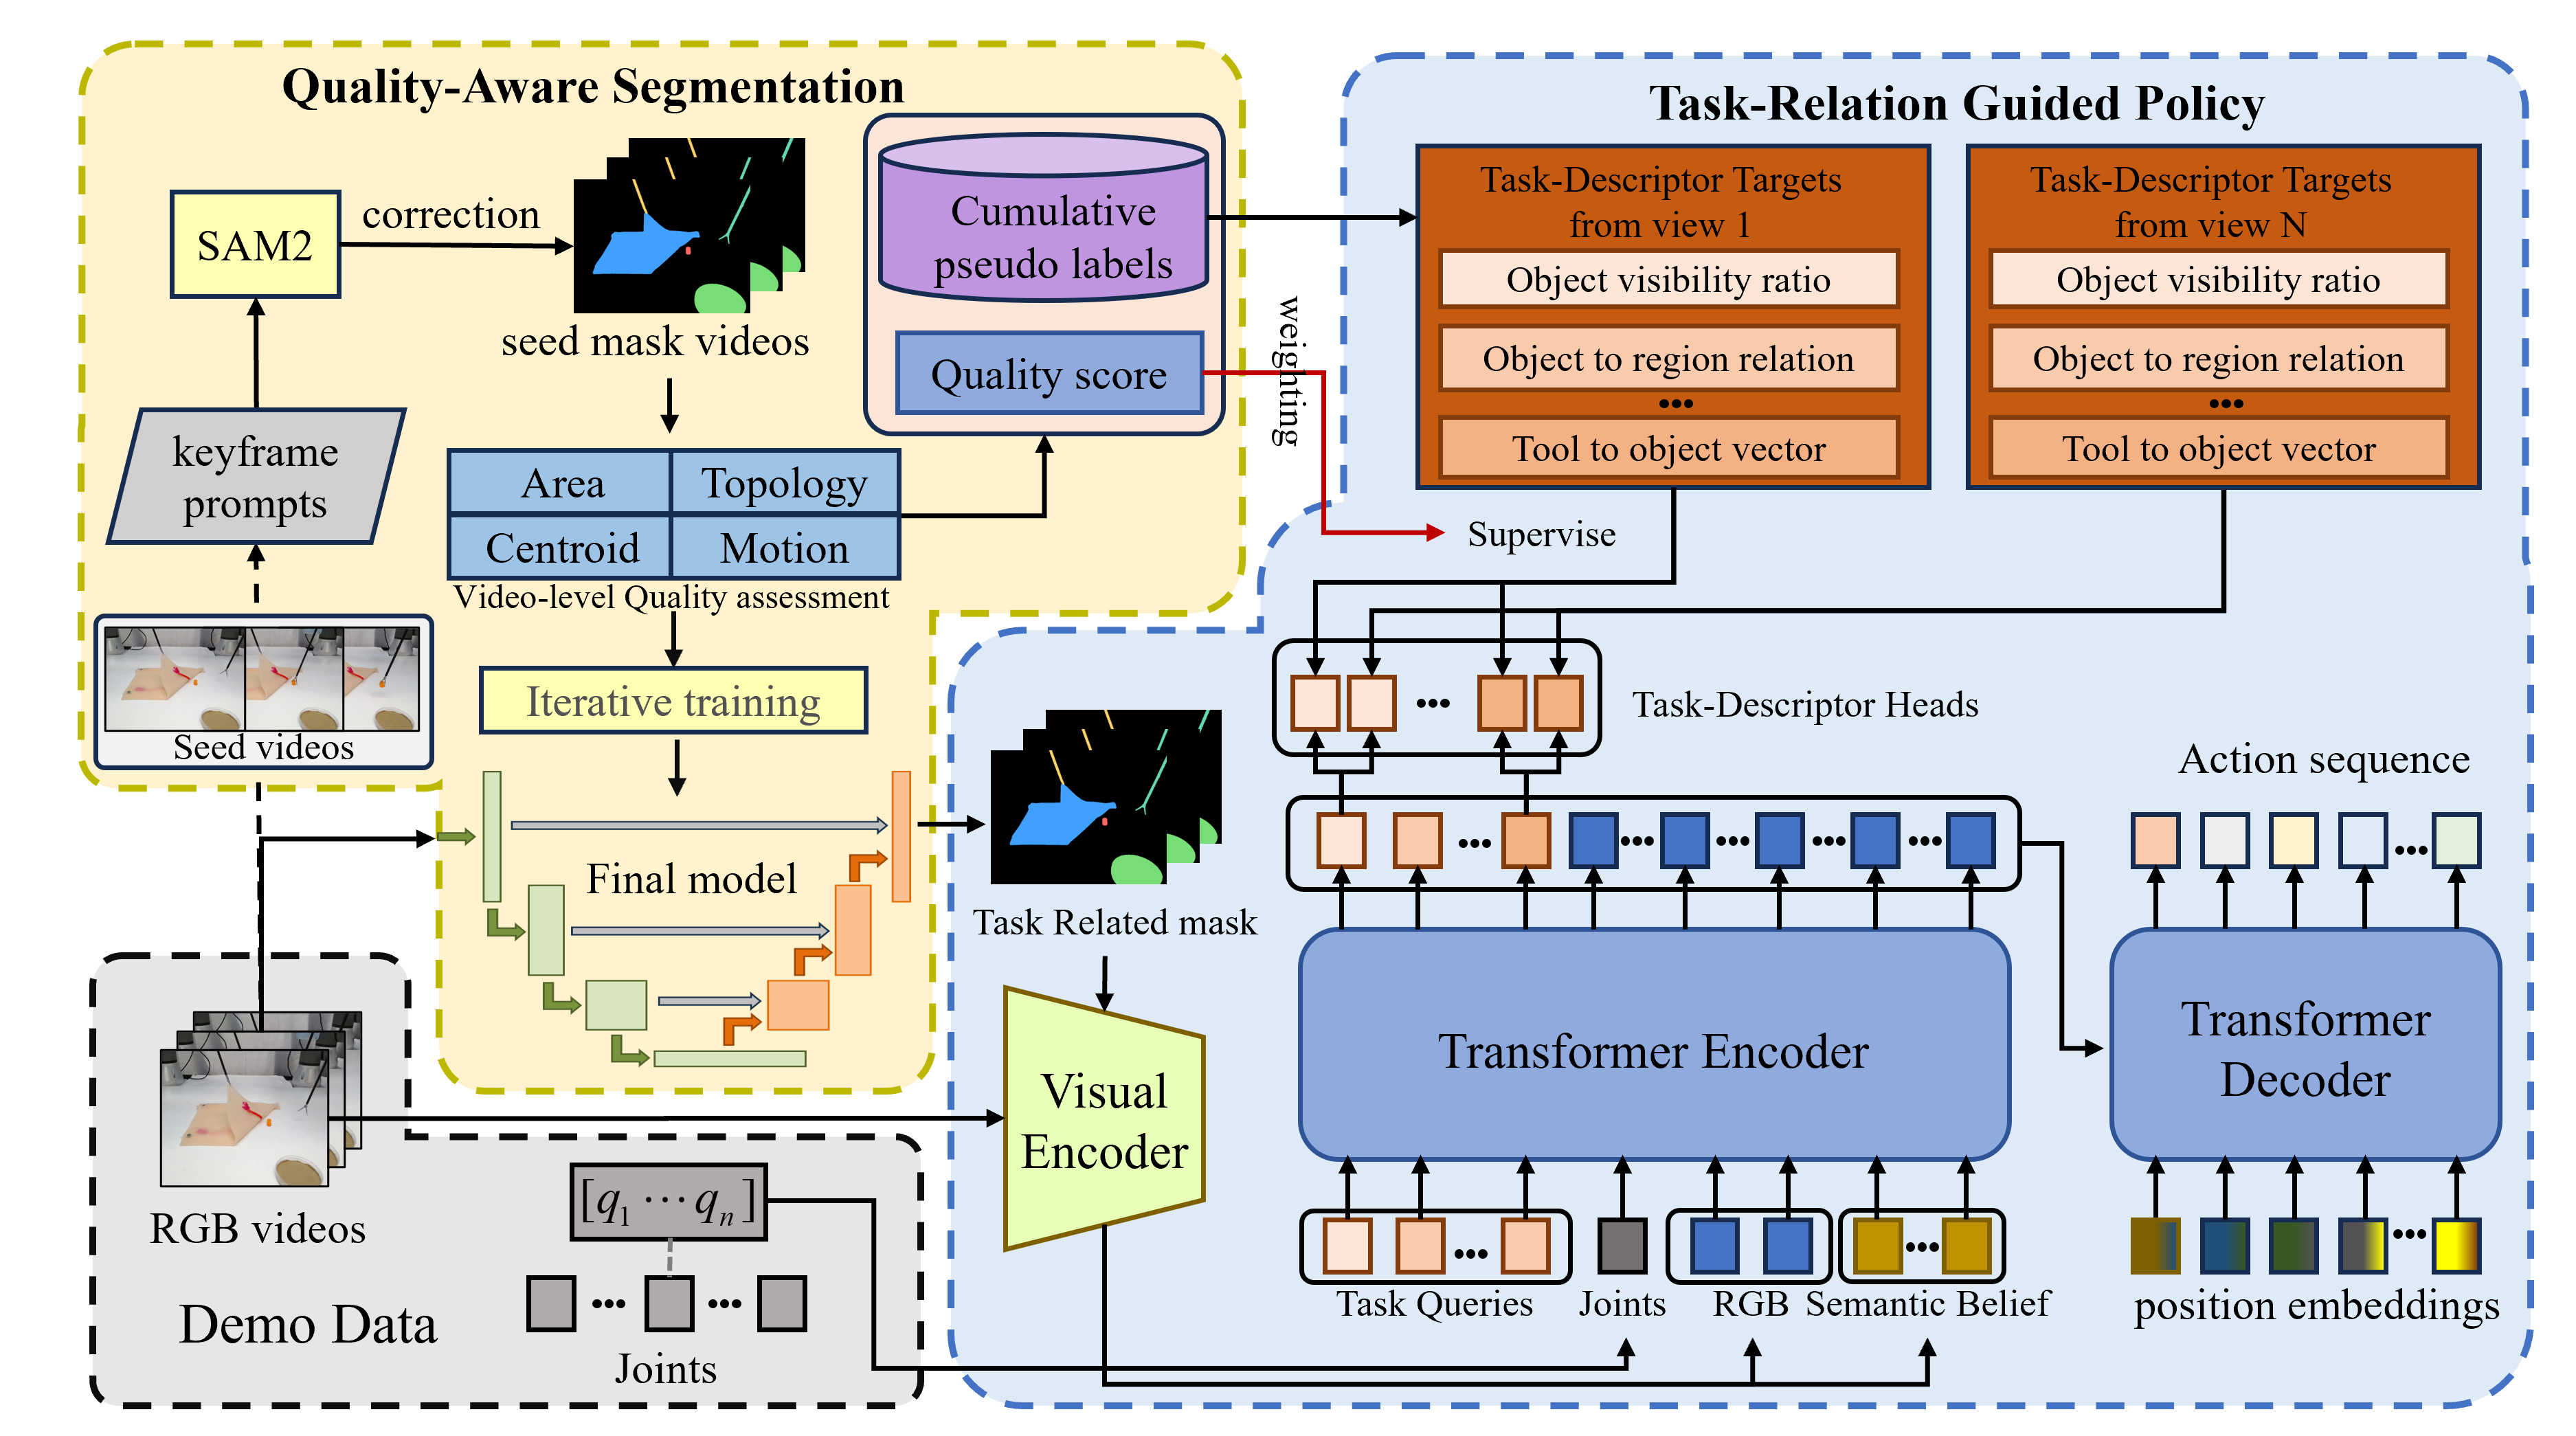
\includegraphics[width=\textwidth]{myfigure/fig1.png}
\caption{Method overview. Quality-aware cumulative annotation provides frozen per-view segmenters, task-descriptor targets, and reliability weights. A shared visual backbone encodes the RGB and semantic streams. One learned query per task relation integrates visual and proprioceptive information, is supervised by independent view-specific heads, and remains available to the action decoder for action-chunk prediction.}
\label{fig:architecture}
\end{figure*}


\section{Method}
\label{sec:method}
Section~\ref{sec:analysis} motivates a policy representation that preserves the task conditions needed for expert bimanual action selection.
Our framework implements this principle through three connected components, as summarized in Fig.~\ref{fig:architecture}.
First, a task-relation policy transformer combines RGB observations, semantic structure, proprioception, and supervised task queries to predict action chunks.
Second, quality-aware iterative semantic supervision expands a small reviewed seed set without repeatedly invoking a video foundation model.
Third, mask-derived task descriptors supervise the query representation according to the reliability of the semantic evidence from which each descriptor is computed.

\subsection{Task-Relation Policy Transformer}
\label{sec:methodpolicy}
The policy assigns complementary roles to semantic inputs and task-query supervision.
Semantic images expose object-level structure and changes in the deformable occluder to the visual encoder.
Task queries directly supervise selected decision variables in the representation used for action generation.
RGB and proprioception retain appearance, contact, deformation, and robot-configuration cues not captured by category masks.

\subsubsection{Joint RGB-Semantic Encoding}
For each camera view $v$, a frozen segmenter maps the RGB image $I_t^v$ to a class map containing the occluder, target object, goal region, tool, and two robot arms.
Class-dependent component filtering removes small or excess connected components, after which a fixed color palette converts the class map into a three-channel semantic image $S_t^v$.
Policy training uses offline semantic masks from the expanded semantic dataset, while deployment applies the frozen segmenters to the current RGB observations.

Each RGB and semantic stream is processed independently by the shared ACT visual backbone~\cite{zhao2023act}.
The resulting visual tokens are combined with the two-arm proprioceptive state and a set of learned task-query tokens in the transformer encoder.
The ACT decoder attends to the complete encoder memory and predicts a coordinated action chunk.
Thus, the semantic stream exposes changes such as target revelation, occluder displacement, and tool motion without replacing the appearance information in RGB.

\subsubsection{Shared Task Queries and View-Specific Heads}
We use one learned query for each of three task relations: target visibility, tool--target displacement, and target--goal-region distance.
Let $z_t^{(j)}$ denote the encoder output of query $j$.
The same query representation is read by independent heads for the front and side views,
\begin{equation}
 \widehat G_t^{(j,v)}=D_{j,v}\!\left(z_t^{(j)}\right).
 \label{eq:viewqueryheads}
\end{equation}
The shared query integrates complementary evidence across views, while view-specific heads preserve quantities defined in different image coordinates.
The encoded query tokens remain in the encoder memory attended by the action decoder.
Descriptor predictions provide auxiliary supervision and are not appended to the policy input.

\subsection{Quality-Aware Iterative Semantic Supervision}
\label{sec:methodseg}
The semantic images and descriptor targets both depend on mask quality.
We therefore expand the mask annotations through cumulative self-training while screening transient segmentation failures at the video level.

\subsubsection{Reviewed Seeds and Cumulative Expansion}
We first choose a small set of videos that spans key interaction states, including initial occlusion, target exposure, tool contact, placement, and covering restoration.
Bounding boxes and positive and negative point prompts are placed on event-centered keyframes.
Bidirectional Segment Anything Model 2 (SAM2) propagation~\cite{ravi2024sam2}, forward--backward consistency checks, and manual correction produce the reviewed seed mask videos.
The remaining training episodes are task-stratified, randomized, and divided into three disjoint batches.
Each round after the first introduces approximately twice as many new episodes as the preceding round.
The seed episodes and a frozen episode-level benchmark are excluded from the pseudo-label pool.
Algorithm~\ref{alg:iterative-semantic-annotation} summarizes the cumulative expansion.
The benchmark tracks cross-generation segmentation performance.

\begin{figure}[t]
\refstepcounter{troalgorithm}
\label{alg:iterative-semantic-annotation}
\small
\hrule
\vspace{2pt}
\noindent\textbf{Algorithm \thetroalgorithm: Quality-Aware Cumulative Annotation}
\vspace{2pt}
\hrule
\vspace{2pt}
\begin{tabular}{@{}l@{\ }>{\raggedright\arraybackslash}p{0.82\columnwidth}@{}}
\textbf{Input:} & seed masks $\mathcal S_0$, video batches $\mathcal B_{1:K}$, and benchmark $\mathcal E_{\mathrm{seg}}$\\
\textbf{Output:} & segmenter $f_K$ and quality records $\mathcal Q$\\
\end{tabular}
\begin{algorithmic}
\STATE $f_0\leftarrow\operatorname{Train}_{\mathrm{ImageNet}}(\mathcal S_0)$, $\mathcal S\leftarrow\varnothing$, $\mathcal Q\leftarrow\varnothing$
\FOR{$k=1,\ldots,K$}
 \STATE $\widetilde{\mathcal M}_k\leftarrow\operatorname{Predict}(f_{k-1},\mathcal B_k)$
 \STATE $(\bm\upsilon_k,\bm q_k)\leftarrow\operatorname{Quality}(\widetilde{\mathcal M}_k)$
 \STATE $\mathcal A_k\leftarrow\{t:\exists c,v,\alpha_{t,c,v}=1\}$
 \STATE $\mathcal R_k\leftarrow\operatorname{Dilate}\!\left(
 \mathcal A_k\cup\operatorname{GateFail}(\widetilde{\mathcal M}_k)\right)$
 \FOR{$t\in\mathcal B_k$}
  \IF{$t\notin\mathcal R_k$}
   \STATE $\mathcal S\leftarrow\mathcal S\cup\{\widetilde{\mathcal M}_{k,t}\}$, $\mathcal Q\leftarrow\mathcal Q\cup\{\bm q_{k,t}\}$
  \ENDIF
 \ENDFOR
 \STATE $f_k\leftarrow\operatorname{Train}_{\mathrm{ImageNet}}(\mathcal S)$
 \STATE $\operatorname{Evaluate}(f_k,\mathcal E_{\mathrm{seg}})$
\ENDFOR
\end{algorithmic}
\hrule
\end{figure}
Here, $\operatorname{Train}_{\mathrm{ImageNet}}$ denotes training a per-view ResNet U-Net initialized with ImageNet-pretrained encoder weights.
$\operatorname{GateFail}$ denotes excessive structural correction or insufficient foreground, while $\operatorname{Dilate}$ extends each rejected frame to a short temporal neighborhood.

\subsubsection{Video-Level Quality Screening}
Framewise confidence alone conflates genuine task transitions with transient segmentation errors.
For each semantic class $c$ and view $v$, we therefore analyze complete-video trajectories using four evidence groups:
mask area, spatial shape from centroid and bounding-box changes, topology from connected components and holes, and motion consistency from flow-aligned mask overlap.
Area reveals sudden disappearance or expansion.
Centroid and bounding-box trajectories expose implausible location or extent jumps.
Connected components, hole counts, and hole area reveal fragmentation or merging that area alone can miss.
For motion, we compute $I_{t,c,v}$, the intersection over union between the current mask and the preceding mask warped through forward--backward-consistent optical flow.
A drop below its robust expected value gives the motion deviation $d_{t,c,v}^{\mathrm{motion}}=[\widehat I_{t,c,v}-I_{t,c,v}]_+$.
Missing or unreliable flow supplies no motion evidence.

Each continuous diagnostic is compared with a piecewise robust temporal trend so that a persistent change, such as deliberate occluder displacement or target exposure, establishes a new state.
Let $d_{t,c,v}^{g}$ be the resulting normalized deviation for evidence group $g$, and let $\rho_{t,c,v}^{g}$ be its local median absolute residual scaled by $1.4826$.
The excess over the group-specific tolerance $\epsilon_g$ is
\begin{equation}
 \upsilon_{t,c,v}^{g}
 =\left[
 \frac{d_{t,c,v}^{g}}
 {\max(\epsilon_g,\kappa\rho_{t,c,v}^{g})}-1
 \right]_+,
 \qquad \kappa=4,
 \label{eq:qualityevidence}
\end{equation}
where $[u]_+=\max(0,u)$.
Component- or hole-count mismatches directly contribute positive topology evidence.
The four evidence magnitudes define the class-specific quality score
\begin{equation}
 q_{t,c,v}^{\mathrm{seg}}
 =\exp\!\left[-\min\!\left(\tau,
 \sum_g\upsilon_{t,c,v}^{g}\right)\right],
 \qquad \tau=4.
 \label{eq:segquality}
\end{equation}
The score equals one when no evidence departs from its expected trend and decreases as the combined deviation grows.
The multi-evidence anomaly decision is $\alpha_{t,c,v}=\ind[\sum_g\ind[\upsilon_{t,c,v}^{g}>0]\ge2]$.
The joint gate in Algorithm~\ref{alg:iterative-semantic-annotation} therefore prevents an isolated area or motion change from invalidating a label.
The score provides a relative reliability weight rather than a calibrated probability of correctness.
All quality assessment is performed offline.
At deployment, the final frozen segmenters use only the current images.

\subsection{Task Descriptors and Reliability-Aware Supervision}
\label{sec:methodrelations}
The task queries retain information that is directly useful for deciding whether to continue exposure, approach the target, or complete placement.
We instantiate this information using target visibility and two spatial relations.
The more detailed occluder configuration remains available through the semantic stream rather than being compressed into an additional scalar descriptor.

\subsubsection{Task-Descriptor Construction}
Let $M_{O,t}^v$, $M_{T,t}^v$, and $M_{R,t}^v$ denote the target-object, tool, and goal-region masks in view $v$ at time $t$.
For an image of width $W_I$ and height $H_I$, let $\bar c_{O,t}^v$ be the normalized target centroid, $\bar r_{T,t}^v$ a normalized tool reference point, $\mathcal P_v$ a fixed goal-region polygon estimated from reliable training masks, and $D_I=\sqrt{(W_I-1)^2+(H_I-1)^2}$.
The descriptor targets are
\begin{equation}
 \begin{aligned}
 \widetilde G_{t}^{(\mathrm{vis},v)}
 &=\frac{|M_{O,t}^v|}{W_IH_I},\\
 \widetilde G_{t}^{(\mathrm{tool},v)}
 &=\clip\!\left(\bar c_{O,t}^v-\bar r_{T,t}^v,-1,1\right),\\
 \widetilde G_{t}^{(\mathrm{goal},v)}
 &=\frac{1}{D_I}\max_{\xi\in M_{O,t}^v}
   \operatorname{dist}(\xi,\mathcal P_v).
 \end{aligned}
 \label{eq:methodgeometry}
\end{equation}
The current goal-region mask determines descriptor validity and mask reliability, while the fixed polygon $\mathcal P_v$ provides a stable spatial reference.
The visible-area ratio measures the degree of target exposure.
The signed two-dimensional displacement preserves the direction from the execution end toward the target.
In the front view, the tool reference is the left endpoint of the tool mask's principal-axis segment.
In the side view, where endpoint orientation is not reliably identifiable, the tool centroid is used.
Distance to $\mathcal P_v$ is zero inside the goal region, so the maximum in~\eqref{eq:methodgeometry} becomes zero only when all visible target pixels lie inside it.
This retains completion-relevant information that a centroid distance could miss.

A reliably empty target mask is a valid zero-visibility label.
The two geometric relations are undefined when their required objects or reference geometry are unavailable, so they are masked rather than assigned a zero value.
These descriptors encode observable image-plane task relations, while unobserved three-dimensional contact and deformation lie outside their scope.

\subsubsection{Descriptor Reliability and Joint Objective}
Mask-derived descriptor targets inherit segmentation errors.
We therefore weight each descriptor using the semantic classes required for its computation.
Let $\mathcal C_j$ be those classes and $m_{t,j,v}^{G}$ indicate that the geometry is defined.
We use
\begin{equation}
 \varpi_{t,j,v}^{G}
 =m_{t,j,v}^{G}
  \prod_{c\in\mathcal C_j}(1-\alpha_{t,c,v})
  \min_{c\in\mathcal C_j}q_{t,c,v}^{\mathrm{seg}}.
 \label{eq:relationadmission}
\end{equation}
Visibility uses target quality.
Tool--target displacement uses the lower of target and tool quality, while target--goal distance uses the lower of target and goal-region quality.
The weighting depends only on the classes required by each descriptor.
Occluder changes therefore leave valid spatial labels active, while the semantic input retains the occluder structure.
An anomaly or undefined relation gives zero auxiliary weight without removing the corresponding action demonstration.

For action supervision, let $u_{n,h,d}^{\mathrm E}$ and $\widehat u_{n,h,d}$ denote the dataset-normalized expert and predicted joint-command components for sample $n$, prediction step $h$, and command dimension $d$.
Let $p_{n,h}\in\{0,1\}$ mask padded steps, $H_a$ be the prediction horizon, $d_u$ be the joint-command dimension, and $N_b$ be the minibatch size.
During training, the conditional variational encoder also represents each demonstrated action sequence by a Gaussian with mean $\mu_n$ and diagonal variance $\sigma_n^2$.

With $V$ views, three descriptor groups, and component-averaged Smooth L1 loss $\ell_G$, the descriptor and complete training objectives are
\begin{align}
 \mathcal L_{\mathrm{rel}}
 &=\frac{1}{3V}\sum_{j,v}
   \frac{\sum_n\varpi_{n,j,v}^{G}
      \ell_G(\widehat G_n^{(j,v)},\widetilde G_n^{(j,v)})}
        {\max(1,\sum_n m_{n,j,v}^{G})},\nonumber\\
 \mathcal L
 &=\frac{1}{N_bH_ad_u}
  \sum_{n=1}^{N_b}\sum_{h=1}^{H_a}\sum_{d=1}^{d_u}
  p_{n,h}\left|\widehat u_{n,h,d}-u_{n,h,d}^{\mathrm E}\right|
  \nonumber\\
 &\quad+\frac{\beta_{\mathrm{KL}}}{2N_b}
  \sum_{n=1}^{N_b}\sum_r
  \left(\mu_{n,r}^{2}+\sigma_{n,r}^{2}
  -\log\sigma_{n,r}^{2}-1\right)
  +\lambda_{\mathrm{rel}}\mathcal L_{\mathrm{rel}}.
 \label{eq:methodbaseloss}
\end{align}
The denominator counts valid descriptor targets rather than the sum of their quality weights, so uniformly uncertain labels reduce the auxiliary gradient instead of being renormalized to full strength.
The segmenters remain frozen during policy learning.
Together, the shared queries, view-specific heads, and reliability-aware objective provide direct supervision for preserving the selected task information in the action-generating representation, as motivated by~\eqref{eq:expertreconstruction}.

\section{Experiments}
\label{sec:experiments}
We evaluate the proposed method in two real-robot bimanual expose--execute--restore tasks: the Surgical-Task Setup and the Daily-Task Setup.
In both setups, the robot must retract a deformable occluder to expose the target, 
execute the target-directed manipulation, and restore the occluder.
To evaluate the proposed framework, our experiments study the following questions.
\begin{enumerate}
    \item Can quality-aware iterative annotation produce large-scale, reliable semantic masks with only a few manual annotations?
    \item Does the proposed method improve complete-task performance over the baselines?
    \item Do these improvements generalize across variations in objects, scenes, and spatial configurations?
    \item How do semantic inputs and task-query supervision each contribute to complete-task performance?
\end{enumerate}

\subsection{Experimental Setup}
\label{sec:experimentalsetup}

\subsubsection{Surgical-Task Setup}
The surgical setup (Fig.~\ref{fig:twosettings}a) uses a dual-UR system to manipulate tissue-mimicking material.
One arm retracts the material to establish visibility and access, while the other grasps the exposed target and transfers it to the designated region.
We evaluate four combinations of two target colors and two spatial layouts, with five independently reset trials per condition and 20 trials per policy.
Each trial has a 180-s horizon, and the saved operator-confirmed outcome determines task success.
All policies share the same robot interface, workspace limits, task-specific demonstrations, and right-gripper fallback configuration.

\subsubsection{Daily-Task Setup}
The daily setting (Fig.~\ref{fig:twosettings}b) uses two SO-ARM101 manipulators and fixed front and side cameras with $640\times360$ images.
The 108 demonstrations contain 61,740 synchronized frames recorded at 30 Hz with 10-dimensional joint states and commands.
The demonstrated objects are a cube, paper ball, and screw.
The test set adds a crayon category absent from the policy demonstrations.
For each of the four objects, we test a $4\times3$ grid of initial positions twice, giving 96 trials per policy and 480 trials across five policies.
A trial succeeds when the object is fully inside the goal region and front-view cloth coverage exceeds 0.32 within 40 s.

\begin{figure}[t]
\centering
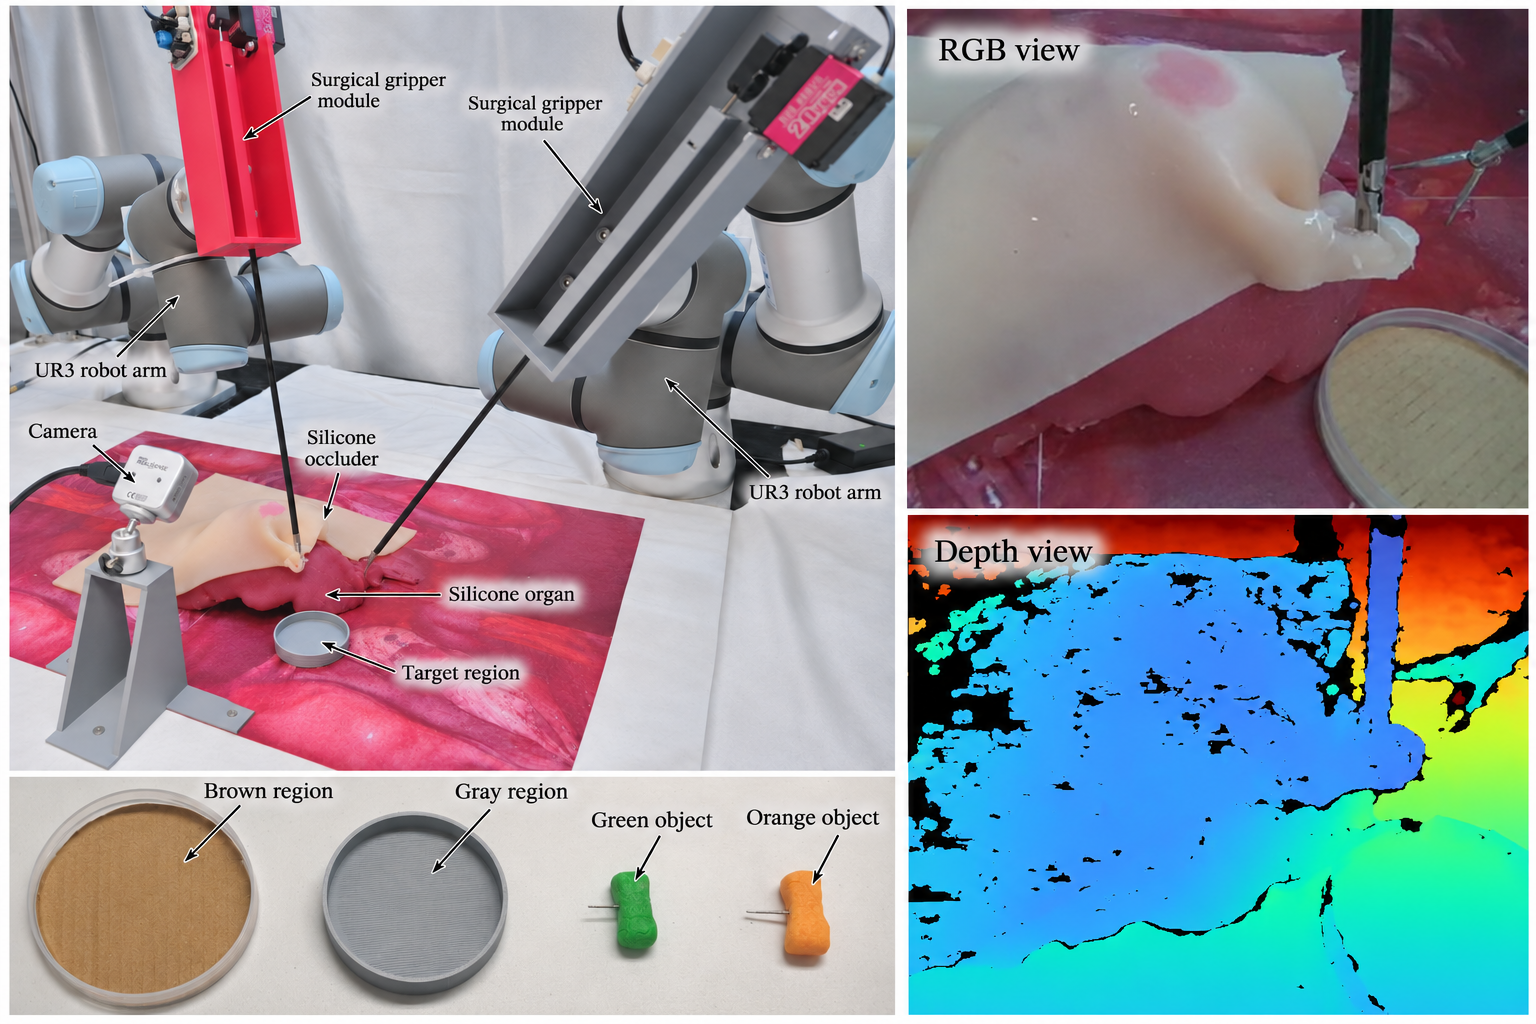
\includegraphics[width=\columnwidth]{myfigure/surgical-task-with-camera-views-v2.png}\par
{\footnotesize (a) Surgical-Task Setup\par}
\vspace{4pt}
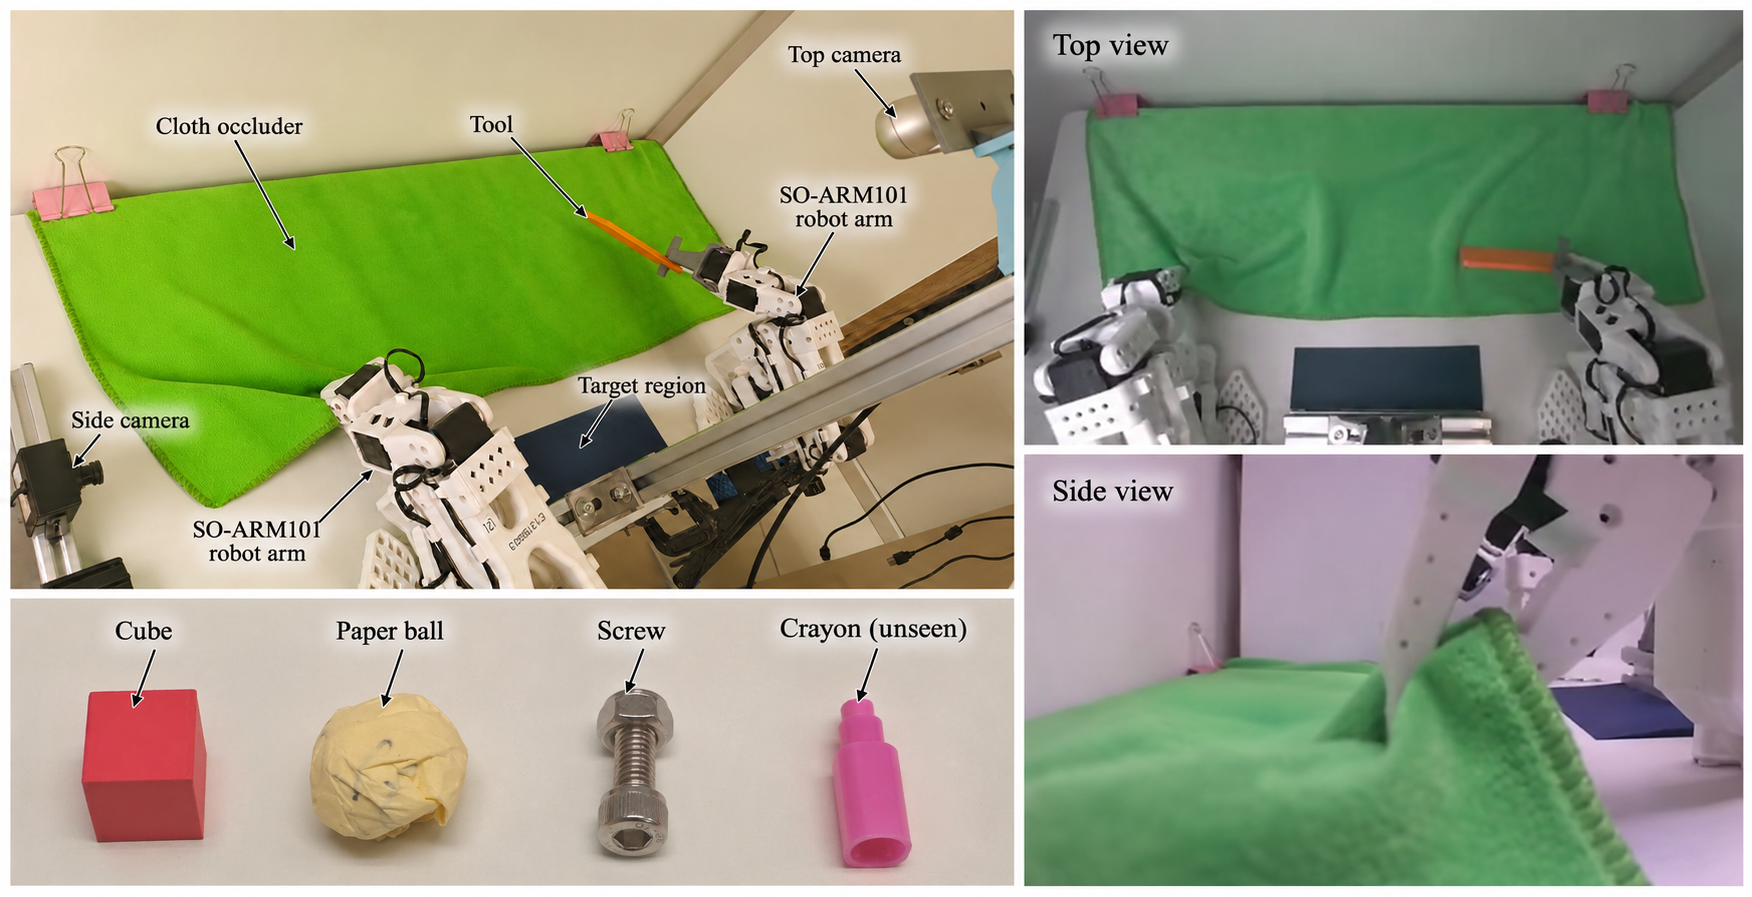
\includegraphics[width=\columnwidth]{myfigure/daily-task-with-camera-views.png}\par
{\footnotesize (b) Daily-Task Setup\par}
\caption{Real-robot experimental setups. (a) Surgical-task setup with two target regions, two colored objects, and RGB and depth views. (b) Daily-task setup with four object categories and top and side views. The crayon category is absent from the policy demonstrations.}
\label{fig:twosettings}
\end{figure}

\subsubsection{Policies and Metrics}
We compare Ours with Action Chunking with Transformers (ACT)~\cite{zhao2023act} and Diffusion Policy (DP)~\cite{chi2023diffusion} in both settings.
The complete task-relation policy is denoted as Ours.
Its controlled variants are named by the removed component: Ours w/o semantic inputs, Ours w/o task-query supervision, and Ours w/o both components, which recovers the ACT backbone.
ACT provides an action-only comparison on the same policy backbone, while DP tests whether an alternative multimodal action-generation objective closes the complete-task gap.
All policies within a setting use the same action demonstrations.
Ours and its controlled variants additionally use the offline semantic supervision specified by their enabled components.

The primary metric is complete-task success.
We also report conditional completion time over successful trials and performance across task conditions, object categories, colors, and initial positions.
Training and deployment configurations are detailed in Appendix~\ref{app:testedimplementation}.

\subsection{Quality-Aware Iterative Annotation}
\label{sec:annotationresults}
\noindent\textbf{Surgical simulation.}
Four reviewed seed videos initialize the front-view segmenter.
Three cumulative generations then train on 8, 24, and 82 quality-screened videos.
A fixed eight-video benchmark contains four anchor videos with reviewed pixel labels and four unseen videos excluded from all training generations.
On the unseen videos, the raw multi-evidence flagged-frame rate decreases from 8.26\% to 3.29\%, while the filtered rate decreases from 2.18\% to 0.54\%.
The anchor foreground mIoU remains stable at approximately 95.4\% across generations, showing that the expansion preserves seed-label agreement while improving temporal and structural consistency on unseen videos.

\begin{table}[t]
\centering
\caption{Surgical-simulation annotation results. Flagged-frame rates decrease on four unseen videos while foreground mIoU remains stable on four reviewed anchor videos.}
\label{tab:surgicalannotation}
\small
\setlength{\tabcolsep}{2.5pt}
\begin{tabular}{lrrrr}
\toprule
Generation & Videos & Raw & Filtered & mIoU\\
\midrule
G1 & 8 & 8.26\% & 2.18\% & 95.45\%\\
G2 & 24 & 6.23\% & 1.12\% & 95.45\%\\
G3 & 82 & 3.29\% & 0.54\% & 95.43\%\\
\bottomrule
\end{tabular}
\end{table}

\noindent\textbf{Daily manipulation.}
Three reviewed seed trajectories train the initial per-view segmenters, and three held-out trajectories track cross-generation performance.
The three cumulative rounds add 15, 29, and 58 new trajectories, yielding 47,766 accepted front-view masks and 42,010 accepted side-view masks in the final pool.

\begin{figure}[t]
\centering
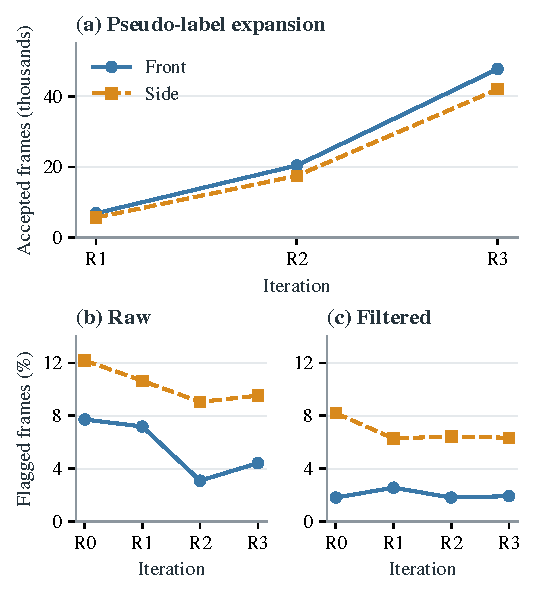
\includegraphics[width=\columnwidth]{figures/annotation_finaldata/annotation_iteration_en.pdf}
\caption{Quality-aware annotation expansion. Accepted supervision increases across rounds, while held-out flagged-frame rates are lower at R3 than at R0 but are not monotonic across rounds.}
\label{fig:annotationiteration}
\end{figure}

On the held-out trajectories, the raw flagged-frame rate decreases from 7.72\% to 4.42\% in the front view and from 12.19\% to 9.53\% in the side view between R0 and R3.
Both views attain their lowest raw rate at R2 rather than R3.
After structural filtering, the side-view rate decreases from 8.20\% to 6.34\%, while the front-view rate changes from 1.81\% to 1.92\%.
The final seed-reference foreground mIoU is 97.87\% for the front view and 97.65\% for the side view.
Across both settings, cumulative self-training expands semantic supervision while maintaining high seed agreement, but increasing the pseudo-label pool does not improve every held-out diagnostic monotonically.

\FloatBarrier

\subsection{Task Evaluation Performance}
\label{sec:overallresults}

\subsubsection{Comparison in the Two Settings}
\noindent\textbf{Surgical simulation.}
Table~\ref{tab:surgicalcomparison} reports results for the two target colors and two spatial layouts.
Ours succeeds in 19 of 20 trials (95.0\%), compared with 8 of 20 (40.0\%) for ACT and 11 of 20 (55.0\%) for DP.
The improvement is consistent across all four evaluated conditions.
Among successful trials, the mean execution time of Ours is 93.12 s, close to ACT at 89.33 s and below DP at 109.62 s.
This conditional comparison evaluates the duration of successful executions rather than overall efficiency across failures.

\begin{table}[t]
\centering
\caption{Surgical-simulation comparison. Ours achieves the highest complete-task success in every color--layout condition. Each condition contains five trials.}
\label{tab:surgicalcomparison}
\small
\setlength{\tabcolsep}{3.2pt}
\begin{tabular}{lccccc}
\toprule
& \multicolumn{2}{c}{Layout A} & \multicolumn{2}{c}{Layout B} & \\
\cmidrule(lr){2-3}\cmidrule(lr){4-5}
Method & Orange & Green & Orange & Green & Overall\\
\midrule
ACT & 2/5 & 1/5 & 2/5 & 3/5 & 8/20\\
DP & 3/5 & 2/5 & 4/5 & 2/5 & 11/20\\
\textbf{Ours} & \textbf{5/5} & \textbf{5/5} & \textbf{5/5} & \textbf{4/5} & \textbf{19/20}\\
\bottomrule
\end{tabular}
\end{table}

\begin{figure}[t]
\centering
\fbox{\parbox{0.92\columnwidth}{\centering\small
\vspace{7pt}
(a) Surgical layout map\\[4pt]
(b) Success by target color and location\\[4pt]
(c) Completion-time distribution
\vspace{7pt}}}
\caption{Condition-level surgical results. The spatial layout, color-wise success, and completion-time plots will replace this placeholder.}
\label{fig:surgicalconditions}
\end{figure}

\noindent\textbf{Daily manipulation.}
Ours succeeds in 92 of 96 trials (95.8\%), improving over ACT and DP by 39.6 and 43.8 percentage points, respectively.
It succeeds in 23 of 24 trials for every object category, including the crayon category absent from the demonstrations.
Among successful trials, its mean completion time is 14.77 s, compared with 14.96 s for ACT and 15.28 s for DP.
When failures are included, the mean control time is 15.82 s for Ours, compared with 25.92 s for ACT and 27.13 s for DP, because most baseline failures reach the 40-s horizon.
This all-trial measure reflects reliability as well as execution speed.
The blocked exact comparisons give Holm-adjusted $p=3.83\times10^{-10}$ against ACT and $p=8.57\times10^{-12}$ against DP.

\begin{table}[t]
\centering
\caption{Daily-manipulation comparison. Ours achieves 23/24 successes in every object category, including the crayon category absent from the policy demonstrations.}
\label{tab:mainresults}
\small
\setlength{\tabcolsep}{3.0pt}
\begin{tabular}{lccccc}
\toprule
Method & Cube & Paper & Screw & Crayon & Overall\\
\midrule
ACT & 18/24 & 12/24 & 11/24 & 13/24 & 54/96\\
DP & 12/24 & 16/24 & 13/24 & 9/24 & 50/96\\
\textbf{Ours} & \textbf{23/24} & \textbf{23/24} & \textbf{23/24} & \textbf{23/24} & \textbf{92/96}\\
\bottomrule
\end{tabular}
\end{table}

Figure~\ref{fig:comparisonpositions} shows the spatial distribution of task success for the comparison methods.
Ours achieves at least 7/8 successes at every grid position, whereas the worst positions of ACT and DP reach only 1/8 and 0/8.
The gains therefore extend across object categories and initial positions rather than concentrating in a small subset of conditions.

\begin{figure}[t]
\centering
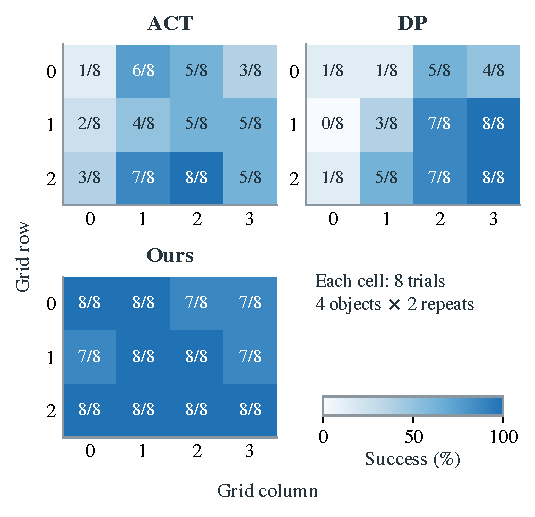
\includegraphics[width=\columnwidth]{figures/results_20261023/position_comparison_en.pdf}
\caption{Spatial comparison in daily manipulation. Ours achieves at least 7/8 successes at every position. Each cell contains eight trials from four objects and two repeats.}
\label{fig:comparisonpositions}
\end{figure}

\subsubsection{Ablation in the Two Settings}
\noindent\textbf{Surgical simulation.}
\draftnote{Insert the surgical ablation results and color--layout analysis.}

\noindent\textbf{Daily manipulation.}
Removing both semantic inputs and task-query supervision gives 54/96 successes.
Retaining only task-query supervision increases success to 72/96, while retaining only semantic inputs gives 60/96.
Combining both components produces the strongest result at 92/96.
Task-query supervision provides the larger standalone gain, increasing success from 54/96 to 72/96 compared with 60/96 from semantic inputs alone.
The larger conditional gains in the combined configurations provide descriptive evidence that the two components are complementary.

\noindent\textbf{Failure-stage analysis.}
ACT and DP leave 34 and 43 trials, respectively, in the separated-but-not-in-region category, compared with 19 for Ours w/o semantics, 31 for Ours w/o task queries, and 4 for Ours.
These labels describe the furthest observed task stage rather than the cause of failure, but show that the main improvement occurs when converting successful exposure and separation into complete transfer.

\begin{figure}[t]
\centering
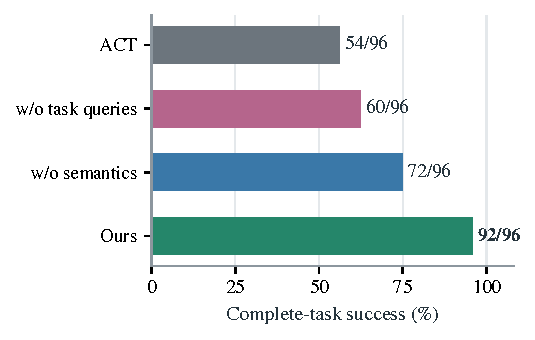
\includegraphics[width=\columnwidth]{figures/results_20261023/ablation_en.pdf}
\caption{Daily-manipulation factorial ablation. Task-query supervision provides the larger standalone gain, while combining both components yields the highest success.}
\label{fig:dailyablation}
\end{figure}

\section{Discussion and Conclusion}
\label{sec:discussion}

\subsection{Discussion}
\noindent\textbf{Task-level reliability.}
The two evaluated settings require later actions to depend on the outcome of earlier interaction with deformable material.
The results show that improving this task-level dependency is not achieved by changing the action generator alone.
ACT and DP frequently produce locally plausible behavior but fail to complete the full sequence, while the proposed representation supervision improves complete-task success across surgical color--layout conditions, daily object categories, and initial positions.
The daily failure-stage results further show that the largest difference occurs after the target has been exposed and separated, when the policy must use the resulting task state to complete transfer.

The factorial ablation clarifies the roles of the two representation components.
Task-query supervision provides the larger standalone gain, which supports directly preserving the relations needed for later decisions.
Semantic inputs alone provide a smaller improvement, showing that object-level visual structure does not by itself ensure that the policy uses the relevant task information.
Their combination performs best, indicating that structured observations and task-directed supervision serve complementary roles.

\noindent\textbf{Semantic supervision.}
The iterative annotation procedure expands a small reviewed set into a substantially larger supervision pool while maintaining high agreement on the reviewed masks.
The held-out flagged-frame rates improve from the initial to the final generation but are not monotonic across rounds.
This distinction is important because label coverage and label consistency are separate properties.
The current experiments evaluate the final annotation and policy pipeline, but do not isolate the contribution of quality screening from the effect of adding more semantic labels.

\noindent\textbf{Residual failures.}
All four daily-manipulation failures of Ours reach target separation but do not complete transfer into the goal region.
The current task descriptors encode visibility and image-plane geometry, but not contact mode, grasp stability, cloth tension, or force interaction.
These unmodeled factors provide concrete targets for extending the task representation.
Quality screening also detects temporal and structural anomalies rather than temporally stable segmentation errors.
The surgical simulation contains one timeout for Ours, while the baseline failures are dominated by workspace-limit and grasping failures.
These outcomes motivate explicit recovery supervision and representations that include contact state.

\begin{figure}[t]
\centering
\fbox{\parbox[c][2.8cm][c]{0.92\columnwidth}{\centering\small
(a) Persistent perception error: RGB, semantic prediction, and reviewed mask\\[4pt]
(b) Correct task descriptors but incomplete transfer: relation state and action trace\\[4pt]
(c) Surgical timeout: exposure, grasp, and transfer stages}}
\caption{Representative residual failure cases to be completed with synchronized observations, task descriptors, and action traces.}
\label{fig:failurecases}
\end{figure}

\noindent\textbf{Scope of the evidence.}
The evaluation uses fixed expert demonstrations and one trained checkpoint per configuration.
The crayon tests measure transfer to an object category absent from the policy demonstrations, but do not establish zero-shot transfer across tasks or robot platforms.
The surgical experiments use tissue-mimicking material and do not constitute clinical validation.
Ours also uses offline semantic supervision beyond the action demonstrations available to ACT and DP.
The theoretical analysis identifies conditions connecting action error, representation coverage, and task failure, while the experiments test the corresponding mechanisms rather than the numerical tightness of the bounds.

\subsection{Conclusion}
This work introduced a task-aware imitation-learning framework for bimanual sequential manipulation from fixed demonstrations.
A quality-aware annotation procedure expands semantic supervision, and supervised task queries preserve target visibility and interaction geometry in the action-generating representation.
The complete method succeeds in 19 of 20 surgical-simulation trials and 92 of 96 daily-manipulation trials, compared with 8 of 20 and 54 of 96 for ACT and 11 of 20 and 50 of 96 for Diffusion Policy.
In the daily factorial study, task-query supervision alone reaches 72 of 96 trials, semantic inputs alone reach 60 of 96, and their combination performs best.
These results demonstrate that explicitly preserving task-relevant state can improve complete-task reliability without additional policy interaction data or an explicit skill selector.
The remaining failures point to contact-aware task descriptors and recovery-focused supervision as the next steps.

% 允许末尾实验浮动体与后续正文自然排版，避免强制清空造成空栏。
\FloatBarrier
\appendices

\section{}
\label{app:actionproofs}
\subsection{Proof of the Policy Performance-Difference Identity}
\label{app:pdidentity}
% 此处动作均为双臂联合指令，终末指标评价完整暴露与执行任务；证明不需要固定阶段划分。
We prove~\eqref{eq:pd} by summing expected changes in the reference value for the complete exposure-and-execution objective.
The evaluation-domain restriction in Section~\ref{sec:task} and
Assumption~\ref{ass:visualassessability} give the terminal value
\begin{equation}
 V_T^{\pi_0}(\mathcal H_T)
 =1-\mathcal V(I_{0:T}^{1:V})=1-\Psi.
 \label{eq:appterminalvalue}
\end{equation}

For $t<T$, taking action $\pi(\mathcal H_t)$ and then following $\pi_0$
gives the failure probability $V_{t+1}^{\pi_0}(\mathcal H_{t+1})$ conditional on the next history.
Averaging over next histories under Assumption~\ref{ass:commonprocess} gives
\begin{equation}
 Q_t^{\pi_0}(\mathcal H_t,\pi(\mathcal H_t))
 =
 \E_\pi\!\left[
 V_{t+1}^{\pi_0}(\mathcal H_{t+1})
 \mid \mathcal H_t
 \right].
 \label{eq:appvaluerecursion}
\end{equation}
Here, $\pi$ determines the next-history distribution, while $V_{t+1}^{\pi_0}$
accounts for subsequent execution under $\pi_0$.

\begin{subequations}
\label{eq:pdproof}
Combining~\eqref{eq:actionconsequence} and~\eqref{eq:appvaluerecursion}
and taking expectations gives
\begin{equation}
 \begin{aligned}
 &\E_\pi[A_t^{\pi_0}(\mathcal H_t,\pi(\mathcal H_t))]\\
 &=\E_\pi\!\left[\E_\pi\!\left[
 V_{t+1}^{\pi_0}(\mathcal H_{t+1})\mid\mathcal H_t\right]\right]
 -\E_\pi[V_t^{\pi_0}(\mathcal H_t)].
 \end{aligned}
 \label{eq:pdproofonestep}
\end{equation}

By the tower property, averaging the conditional next-step value over current histories
gives its unconditional expectation:
\begin{equation}
 \begin{aligned}
 &\E_\pi\!\left[\E_\pi\!\left[
 V_{t+1}^{\pi_0}(\mathcal H_{t+1})\mid\mathcal H_t\right]\right]\\
 &=\E_\pi[V_{t+1}^{\pi_0}(\mathcal H_{t+1})].
 \end{aligned}
 \label{eq:pdprooftower}
\end{equation}

Substituting~\eqref{eq:pdprooftower} into~\eqref{eq:pdproofonestep} and summing over time
leaves only the terminal and initial terms:
\begin{equation}
 \begin{aligned}
 &\E_\pi\sum_{t=0}^{T-1}A_t^{\pi_0}(\mathcal H_t,\pi(\mathcal H_t))\\
 &=\sum_{t=0}^{T-1}\Bigl\{
 \E_\pi[V_{t+1}^{\pi_0}(\mathcal H_{t+1})]-\E_\pi[V_t^{\pi_0}(\mathcal H_t)]\Bigr\}\\
 &=\E_\pi[V_T^{\pi_0}(\mathcal H_T)]-\E_\pi[V_0^{\pi_0}(\mathcal H_0)].
 \end{aligned}
 \label{eq:pdprooftelescope}
\end{equation}

At time $T$, no action remains. By~\eqref{eq:appterminalvalue},
the terminal term is the failure probability under $\pi$:
\begin{equation}
 \E_\pi[V_T^{\pi_0}(\mathcal H_T)]=\E_\pi[1-\Psi]=F(\pi).
 \label{eq:pdproofterminal}
\end{equation}

The policies share the initial-history distribution, so the initial term equals
the failure probability of following $\pi_0$ throughout:
\begin{equation}
 \begin{aligned}
 \E_\pi[V_0^{\pi_0}(\mathcal H_0)]
 &=\E_{\pi_0}[V_0^{\pi_0}(\mathcal H_0)]\\
 &=F(\pi_0).
 \end{aligned}
 \label{eq:pdproofinitial}
\end{equation}

Finally, substituting~\eqref{eq:pdproofterminal} and~\eqref{eq:pdproofinitial}
into~\eqref{eq:pdprooftelescope} gives
\begin{equation}
 \E_\pi\sum_{t=0}^{T-1}A_t^{\pi_0}(\mathcal H_t,\pi(\mathcal H_t))
 =F(\pi)-F(\pi_0).
 \label{eq:pdproofresult}
\end{equation}
\end{subequations}

This establishes~\eqref{eq:pd}.

\subsection{Proof of the Task-Failure Bound}
\label{app:actionriskbound}
We prove~\eqref{eq:successbound} by first bounding task consequences
through action deviations and then transferring the resulting
deployment error to the demonstration distribution.

Set $\pi_0=\pi_{\mathrm E}$ and let $e(h)=\norm{\pi(h)-\pi_{\mathrm E}(h)}$.
\begin{subequations}
\label{eq:riskproof}
Applying Assumption~\ref{ass:actionsensitivity} in~\eqref{eq:pd}
bounds each step's increase in failure probability by its action deviation:
\begin{equation}
 F(\pi)-F(\pi_{\mathrm E})
 \le L\,\E_\pi\!\left[\sum_{t=0}^{T-1}e(\mathcal H_t)\right].
 \label{eq:riskproofsensitivity}
\end{equation}

Since $\bar\mu_\pi$ samples control steps uniformly, the time sum equals
$T$ times the deployment average:
\begin{equation}
 \E_\pi\!\left[\sum_{t=0}^{T-1}e(\mathcal H_t)\right]
 =T\,\E_{(t,h)\sim\bar\mu_\pi}e(h).
 \label{eq:riskprooftimeaverage}
\end{equation}

By the Cauchy--Schwarz inequality, the mean action deviation is bounded
by its root mean square:
\begin{equation}
 \E_{\bar\mu_\pi}e(h)
 \le\sqrt{\E_{\bar\mu_\pi}e(h)^2}.
 \label{eq:riskproofsquared}
\end{equation}

Assumption~\ref{ass:democoverage} also bounds expectations of nonnegative
measurable functions, by simple-function approximation and monotone convergence.
Applying it to $e(h)^2$ and using~\eqref{eq:populationimitationrisk} gives
\begin{equation}
 \E_{\bar\mu_\pi}e(h)^2
 \le C\,\E_\nu e(h)^2=C R_\nu(\pi).
 \label{eq:riskproofcoverage}
\end{equation}
\end{subequations}

Combining~\eqref{eq:riskproofsensitivity}--\eqref{eq:riskproofcoverage}
establishes~\eqref{eq:successbound}.

% \subsection{表示层面迁移界的证明}
\subsection{Proof of the Representation-Level Transfer Bound}
\label{app:representationcoverage}
% 先分离条件误差差异与分布覆盖，再用动作敏感性得到任务界。
We prove~\eqref{eq:representationrisktransfer-main} by separating conditional error discrepancy from distributional coverage, then apply action sensitivity to obtain~\eqref{eq:representationcoveragebound}.

% 沿用B3符号及其可积性和可测条件均值条件。
Let $\mu=\bar\mu_\pi$, with the remaining notation and the integrability and measurable conditional-mean conditions as in Section~\ref{sec:representationcoverage}.
% 表示覆盖保证示范零测集也是部署零测集，因此示范侧条件均值在部署表示下有意义。
Representation coverage ensures that $\nu_Z$-null sets are also $\mu_Z$-null sets, so the demonstration-side conditional mean is well defined for the deployment comparison.

\begin{subequations}
\label{eq:representationrisktransfer}
% 第一步：按表示条件化，将部署误差写成各表示下条件平均误差的平均。
First, conditioning on the representation gives
\begin{equation}
 \E_\mu e(h)^2=\E_{\mu_Z}m_\mu(Z).
 \label{eq:transferconditioning}
\end{equation}

% 第二步：同一表示下部署与示范的误差可能不同，由D_phi控制这一差异。
At the same representation, deployment and demonstration conditional errors can differ. By the definition of $D_\phi$,
\begin{equation}
 \begin{aligned}
 \E_{\mu_Z}m_\mu(Z)
 &\le\E_{\mu_Z}m_\nu(Z)
    +\E_{\mu_Z}|m_\mu(Z)-m_\nu(Z)|\\
 &=\E_{\mu_Z}m_\nu(Z)+D_\phi.
 \end{aligned}
 \label{eq:transferdiscrepancy}
\end{equation}

% 第三步：对非负条件误差应用表示覆盖，再用全期望得到示范总体风险。
Finally, applying representation coverage to the nonnegative function $m_\nu$ and taking the total expectation give
\begin{equation}
 \E_{\mu_Z}m_\nu(Z)
 \le C_\phi\E_{\nu_Z}m_\nu(Z)
 =C_\phi R_\nu(\pi).
 \label{eq:transfercoverage}
\end{equation}
\end{subequations}
% 上述三步建立风险迁移界。任务界沿用A-B的敏感性、时间平均与Cauchy--Schwarz步骤。
Combining~\eqref{eq:transferconditioning}--\eqref{eq:transfercoverage} establishes~\eqref{eq:representationrisktransfer-main}.
Under Assumption~\ref{ass:actionsensitivity}, substituting this result into the sensitivity, time-average, and Cauchy--Schwarz steps~\eqref{eq:riskproofsensitivity}--\eqref{eq:riskproofsquared} yields~\eqref{eq:representationcoveragebound}.

% C的证明：描述量读出误差 -> 专家动作重构 -> 条件误差差异。
\section{Proofs for Task-Relevant Information Preservation}
\label{app:representationproofs}

% \subsection{专家动作重构界的证明}
\subsection{Proof of the Expert-Action Reconstruction Bound}
\label{app:expertreconstruction}
% 固定两种分布与共同读出，用三角不等式证明正文重构界。
We prove~\eqref{eq:expertreconstruction} under the common encoder and readouts of Section~\ref{sec:representationanalysis}, with $\mu=\bar\mu_\pi$.
% 第一步：共同的专家动作近似是Z的可测函数。
Define the common represented expert rule $\widehat a_{\mathrm E}(Z)=g_{\mathrm E}(\widehat G,\chi)$.
% 三角不等式和专家选择假设分别约束两分布上的动作重构误差。
The triangle inequality and Assumption~\ref{ass:expertselection} give, for $\rho\in\{\mu,\nu\}$,
\begin{equation}
 \begin{aligned}
 \E_\rho\norm{\pi_{\mathrm E}-\widehat a_{\mathrm E}}
 &\le \E_\rho\norm{\pi_{\mathrm E}-g_{\mathrm E}(G,\chi)}\\
 &\quad+\E_\rho\norm{g_{\mathrm E}(G,\chi)-g_{\mathrm E}(\widehat G,\chi)}\\
 &\le\epsilon_{\mathrm{sel},\rho}+K_{\mathrm E}\delta_{G,\rho}
 =b_\rho.
 \end{aligned}
 \label{eq:appexpertreconstruction}
\end{equation}


% \subsection{条件误差迁移界的证明}
\subsection{Proof of the Conditional-Error Transfer Bound}
\label{app:relationtransfer}
% 先对比真实动作误差与表示中的共同函数，再用覆盖条件合并两分布的重构误差。
We prove Proposition~\ref{prop:relationtransfer} by comparing actual imitation error with a common function of $Z$, then transferring the demonstration-side reconstruction error through representation coverage.
% 沿用正文的策略和专家读出。
Use $\pi(h)=p(Z)$ and $\widehat a_{\mathrm E}(Z)=g_{\mathrm E}(\widehat G,\chi)$ from Section~\ref{sec:representationanalysis}.
% 第二步：策略和专家近似均只依赖Z，因此其平方距离在两分布中是同一个函数。
Since $\pi(h)=p(\phi(t,h))$, the represented squared error
$\ell_Z(z)=\norm{p(z)-\widehat a_{\mathrm E}(z)}^2$ is the same function of $z$ under both distributions.
% 两个动作距离之和不超过两倍动作集合直径，反三角不等式约束距离之差。
All three actions belong to $\mathcal A$, so the reverse triangle inequality yields
\begin{equation}
 \begin{aligned}
 |e(h)^2-\ell_Z(Z)|
 &\le\bigl(\norm{\pi-\pi_{\mathrm E}}
       +\norm{\pi-\widehat a_{\mathrm E}}\bigr)
       \norm{\pi_{\mathrm E}-\widehat a_{\mathrm E}}\\
 &\le 2B_{\mathcal A}\norm{\pi_{\mathrm E}-\widehat a_{\mathrm E}}.
 \end{aligned}
 \label{eq:appsquarederrorperturbation}
\end{equation}
% 分别在两分布下条件化，公共函数ell_Z留在条件期望之外。
Conditioning separately under each distribution gives
\begin{equation}
 |m_\rho(z)-\ell_Z(z)|
 \le 2B_{\mathcal A}
 \E_\rho[\norm{\pi_{\mathrm E}-\widehat a_{\mathrm E}}\mid Z=z].
 \label{eq:appconditionalexpertapprox}
\end{equation}

% 第三步：插入相同的ell_Z，用表示覆盖迁移示范侧条件误差。
Insert the common function $\ell_Z$ between $m_\mu$ and $m_\nu$ and apply representation coverage to the nonnegative demonstration-side conditional error:
\begin{equation}
 \begin{aligned}
 D_\phi
 &\le\E_{\mu_Z}|m_\mu(Z)-\ell_Z(Z)|\\
 &\quad+\E_{\mu_Z}|m_\nu(Z)-\ell_Z(Z)|\\
 &\le\E_{\mu_Z}|m_\mu(Z)-\ell_Z(Z)|\\
 &\quad+C_\phi\E_{\nu_Z}|m_\nu(Z)-\ell_Z(Z)|\\
 &\le 2B_{\mathcal A}(b_\mu+C_\phi b_\nu).
 \end{aligned}
 \label{eq:apprelationdiscrepancy}
\end{equation}
% 有限表示覆盖使示范侧条件不等式也在部署表示分布下几乎处处成立。
Representation coverage ensures that the demonstration-side conditional inequality also holds $\mu_Z$-almost everywhere.
% 代入B3的任务界即可，无需重复完整结论。
This proves~\eqref{eq:relationdiscrepancybound}.
Substitution into~\eqref{eq:representationcoveragebound} establishes~\eqref{eq:relationtransferfailure}.

\section{Method Details}
\label{app:methoddetails}

\subsection{Descriptor Labels and Quality Weights}
\label{app:seguncertainty}
\label{app:visibilityextension}
% 质量依据描述量所需的类别和几何量传播，避免无关类别影响有效监督。
Descriptor supervision uses the quality evidence relevant to its geometric definition rather than a single frame-wide score.
% 举例说明面积、位置及工具端点依赖不同的分割证据。
Visible area depends primarily on target extent and topology; relative position also depends on the localization of both objects, and a tool-endpoint vector is sensitive to tool shape.
% 类别准入、描述量有效性及软降权共同确定权重。
For descriptor $j$ in view $v$, let $\mathcal C_j$ contain its required classes, $\eta_{t,c,v}^{\mathrm{seg}}$ indicate that class $c$ passes anomaly screening, and $m_{t,j,v}^{G}$ indicate geometric validity.
The supervision weight is
\begin{equation}
 \varpi_{t,j,v}^{G}
 =m_{t,j,v}^{G}
  \prod_{c\in\mathcal C_j}\eta_{t,c,v}^{\mathrm{seg}}\,
  \min_{c\in\mathcal C_j}q_{t,c,v}^{\mathrm{seg}},
 \label{eq:relationadmission}
\end{equation}
% 使用相关类别质量分数最小值，不把诊断分数解释为正确概率。
where $q_{t,c,v}^{\mathrm{seg}}\in[0,1]$ is the exported class-specific quality score.
These diagnostic weights are not calibrated probabilities of correctness.
Area uses object quality; tool--object vectors use object and tool quality; region distance uses object and region quality.
% 分母仅统计几何有效标签，整体降权不会被分母抵消。
Normalization in~\eqref{eq:methodbaseloss} counts geometric validity independently of quality, preserving the attenuation of uniformly uncertain labels.

% 区分不可见与漏分，未定义关系不以零距离填充。
An empty mask supplies a zero-area candidate subject to quality screening; an undetected missed segmentation can still produce an erroneous absence label.
Undefined distances and directions are excluded from the auxiliary loss rather than labeled as zero.
% 缺少光流对应不等价于错误，过度结构修补则不进入分割训练。
Missing optical-flow correspondences provide no motion evidence, whereas excessive structural repair excludes a frame from segmentation training.
% 离线诊断可使用完整视频，但不作为在线可用信息。
Whole-video diagnostics may use later frames offline; they are not supplied to the deployed policy.

\subsection{Pseudo-Label and Descriptor-Readout Errors}
\label{app:pseudolabel}
% 使用与C一致的分布索引，以三角不等式分离拟合与标签误差。
For either evaluation distribution $\rho$ used in Section~\ref{sec:representationanalysis}, inserting the descriptor pseudo-label $\widetilde G$ gives
\begin{equation}
 \delta_{G,\rho}
 \le \E_\rho\norm{\widehat G-\widetilde G}
    +\E_\rho\norm{\widetilde G-G}.
 \label{eq:pseudolabel}
\end{equation}
% 第一项是读出相对标签的误差，第二项是标签本身误差；质量筛选主要针对后者。
The terms separate descriptor fitting from pseudo-label error, motivating quality screening in addition to query supervision.
% 准入后的精度并不代表所有历史，需记录有效率。
When measured only on admitted labels, this comparison concerns the admitted subset; the admission rate is reported alongside the error.

\subsection{Task-Descriptor Instance}
\label{app:descriptorinstance}
% 每个任务查询共享，但双视角几何独立监督，不混合像素坐标。
Our instance uses three task-shared queries with separate front- and side-view heads.
They describe target visibility, tool--target displacement, and target--region distance, producing two, four, and two scalars, respectively.
% 定义图像尺寸、掩码与质心。
For each view, let $M_O^v,M_R^v,M_T^v$ be the object, region, and tool masks in an image of width $W$ and height $H_I$.
The labels are
\begin{equation}
 \begin{aligned}
 \widetilde G^{(1,v)}&=|M_O^v|/(WH_I),\\
 \widetilde G^{(2,v)}&=\clip(\bar c_O^v-\bar r_T^v,-1,1),\\
 \widetilde G^{(3,v)}&=\frac{\max_{\xi\in M_O^v}
       \operatorname{dist}(\xi,\mathcal P_v)}
       {\sqrt{(W-1)^2+(H_I-1)^2}}.
 \end{aligned}
 \label{eq:methodgeometry}
\end{equation}
% 归一化像素坐标，保留方向符号。
Here, $\bar c=(c_x/(W-1),c_y/(H_I-1))$ normalizes a centroid, with rightward and downward positive directions.
% 工具端点由主轴极值及左侧约定确定，不等同于物理接触端。
For the front view, $\bar r_T^v$ is the left endpoint of the tool mask's principal-axis segment in normalized coordinates; for the side view, it is the tool centroid.
% 固定区域从训练标注估计；最大像素距离在可见目标完全入区时为零。
The fixed polygon $\mathcal P_v$ is estimated offline from training masks.
Distance is zero inside this polygon, so the third descriptor vanishes when every visible object pixel is inside.
Its label requires nonempty object and region masks; the vector requires a nonempty object mask and a valid tool reference.
Image-plane containment of visible pixels does not establish containment of an occluded physical object.

\subsection{Evaluation Scope}
\label{app:datascope}
% 种子见过初始教师，作为参考而非独立最终测试。
Seed videos used by the initial segmenter provide a development reference, not an independent final test.
% 跨视频分割评价隔离拟合；独立最终测试还需隔离模型选择。
Cross-video segmentation evaluation excludes annotation-training videos; an independent final test also excludes model selection.
% 描述量泛化评价还需隔离策略训练视频，并采用部署模式。
Descriptor-generalization evaluation additionally excludes policy-training videos and uses the base policy in deployment mode.
For ACT, this sets the latent input to zero rather than conditioning on the demonstrated action posterior~\cite{zhao2023act}.

\section{Evaluation and Implementation Details}
\label{app:evalaudit}

\subsection{Statistical Protocol}
The daily-manipulation evaluation contains 480 valid trials, comprising 96 trials for each of five policies.
Every policy is evaluated on four objects, 12 initial positions, and two repeats per object--position condition.
The resulting object--position--repeat grid contains no missing or duplicated entries.

Pairwise comparisons use the 48 object--position conditions as blocks.
Within each block, the exact null distribution reallocates the four binary outcomes of the two compared policies while preserving the block total.
The block distributions are convolved to obtain the exact distribution of the overall success-count difference.
Holm correction is applied to the ten pairwise policy comparisons.
The evaluation uses one trained checkpoint per configuration, so trial repeats quantify execution variability rather than training-seed variability.
The surgical simulation contains 20 trials per policy and is interpreted descriptively across the four color--layout conditions.

\subsection{Tested Policy Configuration}
\label{app:testedimplementation}
Semantic configurations add two hard semantic maps while retaining RGB and proprioception.
Query configurations add three tokens with quality-weighted supervision for target visibility, tool--target displacement, and target--goal distance in both views.
Their geometric definitions are given in~\eqref{eq:methodgeometry}.

Training uses offline masks, while deployment uses the argmax outputs of the frozen U-Net segmenters after structural filtering.
The Smooth L1 query loss uses $\beta=0.01$.
Each view-specific head is normalized by its valid geometric components before the six head losses are averaged.
The supervision weight is the minimum quality score of the relevant classes and becomes zero when a required class is anomalous or the descriptor is undefined.
Action supervision remains active when descriptor supervision is unavailable.

The four ACT-family configurations share demonstrations, 100,000 optimization steps, a batch size of 8, a learning rate of $10^{-5}$, $\beta_{\mathrm{KL}}=10$, and random seed 1000.
Configurations with task-query supervision use $\lambda_{\mathrm{rel}}=1$.
At deployment, the ACT-family policies predict 60 steps and execute 30 before synchronous replanning.
DP uses its diffusion objective and asynchronous deployment configuration.
The crayon evaluation uses 24 DDIM steps, compared with 16 for the demonstrated object categories.

% 排完附录浮动体后再开始参考文献，避免跨栏图混入文献列表。
\clearpage
\bibliographystyle{IEEEtran}
\bibliography{references}
\end{document}
